\documentclass[12pt,twoside]{book}
\usepackage[spanish]{babel}
\decimalpoint
\usepackage[utf8]{inputenc}
\usepackage{cmap}
\usepackage[T1]{fontenc}

\usepackage[margin=1in]{geometry}
\usepackage{amsfonts}
\usepackage{dsfont}
\usepackage{physics} %indispensable
\usepackage{xcolor} %colores, notas
\usepackage{tikz-cd} %para diagrama conmutativo
\usepackage{multicol} %para la lista de operadores
\usepackage{hyperref} %para referencias clickeables
\usepackage{caption}
\usepackage{subcaption}
\usepackage{pdfpages} % para la portada

%==============================
%========== Comandos ==========
%==============================
\newcommand{\mcU}{\mathcal{U}}
\newcommand{\mcV}{\mathcal{V}}
\newcommand{\mcO}{\mathcal{O}}
\newcommand{\mcI}{\mathcal{I}}
\newcommand{\mcL}{\mathcal{L}}
\newcommand{\mcS}{\mathcal{S}}
\newcommand{\hilbert}{{\sf H}}
\newcommand{\mcB}{\mathcal{B}}
\newcommand{\mcH}{\mathcal{H}}
\newcommand{\mcF}{\mathcal{F}}
\newcommand{\mcC}{\mathcal{C}}
\newcommand{\mcT}{\mathcal{T}}
\newcommand{\mcE}{\ensuremath{\mathcal{E}} }
\newcommand{\mcG}{\ensuremath{\mathcal{G}} }
\newcommand{\mcM}{\mathcal{M}}
\newcommand{\mcN}{\mathcal{N}}
\newcommand{\nnn}{\mathcal{N}}
\newcommand{\choi}{\ensuremath{\mcD} }
\newcommand{\mmm}{\mathcal{M}}
\newcommand{\sss}{\mathcal{S}}
\newcommand{\mcD}{\mathcal{D}}
\newcommand{\mcA}{\mathcal{A}}
\newcommand{\mcP}{\mathcal{P}}
\newcommand{\ie}{i.e.}
\newcommand{\Complex}{\mathbb{C}} %Para escribir al espacio de hilbert complejo
\newcommand{\Id}{\mathds{1}}% Para escribir el op. indentidad con notación chida
\newcommand{\CG}[1]{\mcC\left[#1\right]}
\newcommand{\Fuzzy}[1]{\mcF\left[#1\right]}
\newcommand{\nota}[1]{{\color{red} [#1]}}
\newcommand{\notaAd}[1]{{\color{gray} [#1]}} %Notas pero mías
%%Fixnote
\newcommand{\pauli}[1]{\sigma_{#1}} %Para las matrices de pauli
\newcommand{\paulivec}[1]{\hat{#1}\cdot\vec{\sigma}} %Para vectores de Pauli unitarios
\newcommand{\cnot}{\text{C}_{\text{X}}} %Para el CNOT
\newcommand{\purity}[1]{\text{Pu}(#1)} %la pureza
\newcommand{\Abs}{\text{abs}} %abs
\newcommand{\rfroml}{f} %la función r(lambda)
\newcommand{\densityspace}[1]{\mcS(\hilbert_{#1})} %el espacio de operadores de densidad
\newcommand{\unitaryspace}[1]{\text{U}(\hilbert_{#1})} %el espacio de operadores unitarios
\newcommand{\obspace}[1]{\mcL(\hilbert_{#1})} %el espacio de observables
\DeclareMathOperator*{\Motimes}{\text{\raisebox{0.25ex}{\scalebox{0.8}{$\bigotimes$}}}} %para los productos tensoriales
\usepackage[draft,inline,nomargin]{fixme} \fxsetup{theme=color}
\newcommand\dsone{\mathds{1}}
\FXRegisterAuthor{ac}{acc}{\color{red}AC}
\FXRegisterAuthor{dd}{ddg}{\color{blue}DD}
\FXRegisterAuthor{cp}{acp}{\color{orange}CP}

\title{Dinámica de un sistema de dos qubits bajo un modelo de grano grueso}
\author{Adán Castillo Guerrero}
\date{\today}

\begin{document}

\maketitle
\tableofcontents
\newpage
\chapter{Resultados generales}

\section{Diferentes formas de abordar la dinámica}
El objetivo de la tesis es contruir y estudiar ``dinámicas gruesas'', $\Gamma_t$,
\begin{align*}
\Gamma_{t}:&\mcS(\hilbert_2)\rightarrow \mcS(\hilbert_2)\\
&\rho(0) \mapsto \rho(t).
\end{align*}
La dinámica gruesa puede verse como una composición
\begin{equation*}
\Gamma_t:=\mcC \circ \mcU_t \circ \mcA_\mcC.
\end{equation*}
ilustrable a través del siguiente diagrama
\[\begin{tikzcd}[arrows={<-|}]
\rho(0)  & \rho(t) \arrow{l}{\Gamma_{t}} \arrow{d}{\mcC}\\
\varrho(0) \arrow{u}{\mcA_{\mcC}} & \varrho(t). \arrow{l}{\mcU_{t}}
\end{tikzcd}
\]
Si la evolución subyacente total es una operación unitaria $\mcU$, entonces $\mcU_{t}$  denota exactamente $\mcU^{t}$. De esta forma, $\mcU_{t=0}=\Id$, mientras que  $\mcU_{t=1}=\mcU$. De esta forma es que se introduce la dependencia de la variable temporal en $\rho$:
\begin{equation*}
\rho(t)=(\mcC \circ \mcU_t \circ \mcA_\mcC)\rho(0)
\end{equation*}
En esta discusión, $\mcA_\mcC$ denota una aplicación que asigna un estado fino $\varrho(0)$ al estado $\rho(0)$. Esta asignación es completamente dependiente del mapeo de grano grueso $\mcC$. Exploramos dos formas de hacerla. La primera de ellas consiste en definir $\varrho(0)$ como el promedio sobre todos los estados compatibles con $\rho(0)$~\cite{Macro-To-Micro}, es decir
$$\varrho(0)=\overline{\Omega(\rho(0))},$$
donde
\begin{equation*}
\Omega(\rho)=\{\dyad{\psi}\in \mcS(\hilbert_2 \otimes \hilbert_2) \mid \mcC\left[\dyad{\psi}\right]=\rho\}.
\end{equation*}
A esta asignación la llamaremos \textit{asignación promedio}. La segunda forma de asignación consiste en usar el principio de máxima entropía, dados los promedios de un conjunto de observables tomográficamente completo del sistema al nivel grueso. Esto es, asignaremos al estado $\rho_g(0)$ un estado fino que formalmente sea totalmente imparcial y no añada ninguna cantidad de información arbitraría además de las restricciones $\langle A_i \rangle=\tr \left[ A_i \rho_g(0) \right]$, donde el conjunto $\left\{A_i \right\}$ es tomográficamente completo~\cite{jaynes}. A esta asignación la denotaremos como \textit{asignación MaxEnt}. Cabe señalar que por entropía, nos referimos a la entropía de Von Neumann, $S(\rho)=\tr \left[ -\rho \log(\rho) \right]$.

\section{Sobre el dominio de la dinámica y la matriz de correlaciones}

\subsection{Dominio}

El objeto de esta primera tarea era caracterizar el \textit{dominio} de una dinámica $\Gamma_{t}$, como se menciona en el artículo \cite{CGEmergingDynamics}.

Para comenzar, consideremos la dinámica  $\Gamma_{t}$ caracterizada por una evolución subyacente $\mcU_{
t}$, un estado fino inicial $\psi_{0}$, nuestra aplicación de grano grueso $\mcC$, y el estado grueso $\rho_{0}$. Si se asume que el estado grueso es puro, entonces lo siguiente es cierto:
\begin{itemize}
\item $\rho_{0}$ está completamente descrito por dos ángulos $\theta$ y $\phi$
\item $\rho_{0}$ tiene vector de Bloch $\vec{\alpha}=(\cos{\phi}\sin{\theta},\sin{\phi}\sin{\theta},\cos{\theta})$
\item $\psi_{0}=\rho_{0}\otimes\rho_{0}$
\end{itemize}
Ahora, si se expande a $\psi_{0}$ en la base de Pauli,
\begin{equation}
    \psi_{0} = \frac{1}{4}\,\sum_{i,j} \tr[\psi_{0}(\sigma_i \otimes \sigma_j)]\, \sigma_i\otimes\sigma_j
\end{equation}
es relativamente sencillo ver que:
\begin{equation}
    \CG{\psi_{0}} = \frac{1}{2}\qty[\Id + \sum_{i=1}^3[p\gamma_{i,0}+(1-p)\gamma_{0,i}]\sigma_i]
\end{equation}
donde $\gamma_{ij} \equiv \tr[\rho(\sigma_i \otimes\sigma_j)]$. 

Los coeficientes $\gamma_{ij}$ corresponden a las componentes del vector de Bloch de $\psi_{0}$, siendo $\gamma_{i,0}$ y $\gamma_{0,i}$ las componentes de los vectores de Bloch de los subsistemas de $\psi_{0}$. Como $\psi_{0}=\rho_{0}\otimes\rho_{0}$, entonces $\gamma_{i,0}=\gamma_{0,i}=\alpha_{i}$, y se recupera $\CG{\psi_{0}}=\rho_{0}$

Retomando el tema de la tarea, como se menciona en el artículo \cite{CGEmergingDynamics}, para fijar la dinámica y modificar únicamente al estado grueso inicial (esto es, deben modificarse $\vec{\alpha}$).\\
Así, en el espacio de vectores de Bloch $\vec{\gamma}$ se definen tres restricciones correspondientes a tres hiperplanos:
\begin{align}
\alpha_{i}=\Tr[\CG{\psi_{0}}\sigma_{i}]=p\gamma^{i}+(1-p)\gamma^{i+3}=r_{i}
\end{align}
Los vectores normales a estos hiperplanos son nulos en todas sus componentes, exceptuando la $i$-ésima y la $i+3$-ésima, en las que valen $p$ y $(1-p)$ respectivamente. En principio, el dominio de una $\Gamma_{t}$ fija tiene la forma:
\begin{align}
\psi=&\frac{1}{4}\left( \Id_{4}+\vec{\gamma}\cdot\vec{\sigma_{4}} \right)\\
\vec{\gamma}=&\vec{\gamma_{0}}+\sum_{i}c_{i}\vec{v_{i}}\label{eq:newgamma}
\end{align}
donde $\vec{v_{i}}$ son los vectores normales y $c_{i}$ son componentes tales que $\vec{\gamma}$ es un vector de Bloch válido. Si quisiéramos escribir la ecuación (\ref{eq:newgamma})  componente por componente el resultado sería:
\begin{equation}
\vec{\gamma}=\begin{pmatrix}
\alpha_{1}\\
\alpha_{2}\\
\alpha_{3}\\
\alpha_{1}\\
\alpha_{2}\\
\alpha_{3}\\
\alpha_{1}^{2}\\
\alpha_{1}\alpha_{2}\\
\alpha_{1}\alpha_{3}\\
\alpha_{2}\alpha_{1}\\
\alpha_{2}^{2}\\
\alpha_{2}\alpha_{3}\\
\alpha_{3}\alpha_{1}\\
\alpha_{3}\alpha_{2}\\
\alpha_{3}^{3}\\
\end{pmatrix}+\begin{pmatrix}
c_{1}p\\
c_{2}p\\
c_{3}p\\
c_{1}(1-p)\\
c_{2}(1-p)\\
c_{3}(1-p)\\
0\\
0\\
0\\
0\\
0\\
0\\
0\\
0\\
0\\
\end{pmatrix}\label{eq:newvec}
\end{equation}
Esto puede escribirse como un operador de densidad $\psi$. Tras aplicar el coarse graining el resultado es:
\begin{equation}
    \CG{\psi} = \frac{1}{2}\qty[\Id + \sum_{i=1}^3(\alpha_{i}+pc_{i}(3p-2))\sigma_i]\label{eq:newcoarse}
\end{equation}
Es importante notar que aunque el dominio (\ref{eq:newvec}) vive en un espacio quince dimensional, el movimiento se ve limitado a un espacio cinco dimensional, y la variedad descrita es de únicamente tres dimensiones (una por coeficiente $c_{i}$).

\subsection{Matriz de correlaciones}

El objeto de esta tarea es determinar los coeficientes de correlación como se ven en la ecuación (6) del artículo \cite{CGEmergingDynamics}.


Para el mapeo de coarse graining,
\begin{equation}
\CG{\psi}=\Tr_{B}[p\psi+(1-p)S\psi S^{\dag}]
\end{equation}
se hallan los siguientes operadores de Kraus:
\begin{align}
    K_{1}&=\begin{pmatrix} \sqrt{p}&0&0&0\\0&0&\sqrt{p}&0\end{pmatrix} & K_{2}&=\begin{pmatrix} \sqrt{p}&0&0&0\\0&0&\sqrt{p}&0\end{pmatrix} \\ K_{3}&=\begin{pmatrix} \sqrt{1-p}&0&0&0\\0&\sqrt{1-p}&0&0\end{pmatrix} & K_{4}&=\begin{pmatrix} 0&0&\sqrt{1-p}&0\\0&0&0&\sqrt{1-p}\end{pmatrix}
\end{align}
Utilizando la forma de bloque para el operador que actúa en el sistema extendido dada en \cite{Chuang}, el unitario resultante es:
\begin{equation}
V=\begin{pmatrix}
\sqrt{p}&0&0&0&0&0&0&-\sqrt{1 - p}\\
0&0&\sqrt{p}&0&0&0&-\sqrt{1 - p}&0\\
0&\sqrt{p}&0&0&0&-\sqrt{1 - p}&0&0\\
0&0&0&\sqrt{p}&-\sqrt{1 - p}&0&0&0\\
\sqrt{1 - p}&0&0&0&0&0&0&\sqrt{p}\\
0&\sqrt{1 - p}&0&0&0&\sqrt{p}&0&0\\
0&0&\sqrt{1 - p}&0&0&0&\sqrt{p}&0\\
0&0&0&\sqrt{1 - p}&\sqrt{p}&0&0&0 
\end{pmatrix}
\end{equation}
Debí verificar que esta funcionaba cuando lo hice, todo lo demás queda mal porque la unitaria no quedó.


\section{Una unitaria para gobernarlos a todos}

Un operador unitario se traduce como una rotación en la esfera de Bloch. Entonces dos operadores están relacionados por una unitaria si sus vectores de Bloch tienen la misma norma (esto es, si los operadores tienen la misma norma de Frobenius).

Así, si consideramos un estado sobre el eje z,

\begin{equation}\label{eq:rhoz}
\rho_{z}=\frac{1}{2}\qty(\Id+z\sigma_{z})
\end{equation}

entonces este está relacionado mediante una unitaria a cualquier estado $\rho\in\mcS(\hilbert_2)$ con vector de Bloch $\vec{r}$ tal que $\abs{\vec{r}}=z$.

\subsection{El grueso rotado es igual al grueso del rotado}
Sea $\rho_{z}$ como en (\ref{eq:rhoz}), y sea $\{\varrho_{i}\}_{i=1}^{N}$ un conjunto de estados compatibles que satisfacen la medida de Haar. Además, sea $\rho\in\mcS( \hilbert_2)$ un estado grueso tal que $\abs{\vec{r}}=z$.

\begin{equation}
\Rightarrow \exists U \text{ tal que } U\rho_{z}U^{\dag}=\rho
\end{equation}
\ddnote{esto está escrito un poco al revés, más bien sería así:}
\begin{equation}
U\rho_{z}U^{\dag}=\rho \ \  \forall U\in \text{SU}(2)
\end{equation}

Sea $\mcU=U\otimes U$, $\sigma_{i}'=U\sigma_{i}U^{\dag}$. En las siguientes líneas se muestra que si se rota a todo el conjunto $\{\psi_{i}\}$ usando $\mcU$, lo que se halla es el conjunto fino para el mapeo de asignación de $\rho$. Nótese que la rotación no modifica la distribución de los estados siempre que estos satisfagan la medida de Haar.

\begin{align*}
\CG{\mcU \varrho_{i} \mcU^{\dag}}=&\Tr_{2}\qty[p\mcU\varrho_{i}\mcU^{\dag}+(1-p)S\mcU \varrho_{i} \mcU^{\dag}S^{\dag}]\\
=&\Tr_{2}\qty[p\mcU\qty(\frac{1}{4}\sum_{i,j}\gamma_{ij} \sigma_i\otimes\sigma_j)\mcU^{\dag}+(1-p) S\mcU \qty(\frac{1}{4}\sum_{i,j}\gamma_{ij} \sigma_i\otimes\sigma_j) \mcU^{\dag} S^{\dag}]\\
=&\Tr_{2}\qty[p\qty(\frac{1}{4}\sum_{i,j}\gamma_{ij} \sigma_{i}'\otimes\sigma_{j}')+(1-p)S \qty(\frac{1}{4}\sum_{i,j}\gamma_{ij} \sigma_{i}'\otimes\sigma_{j}')S^{\dag}]\\
=&\Tr_{2}\qty[p\qty(\frac{1}{4}\sum_{i,j}\gamma_{ij} \sigma_{i}'\otimes\sigma_{j}')+(1-p)\qty(\frac{1}{4}\sum_{i,j}\gamma_{ij} \sigma_{j}'\otimes\sigma_{i}')]\\
=&\frac{1}{2}\qty[\Id +p\sum_{i=1}\gamma_{i,0}\sigma_{i}'+(1-p)\sum_{j=1}\gamma_{0,j}\sigma_{j}']\\
\end{align*}
\begin{align*}
\Rightarrow\CG{\mcU \varrho_{i} \mcU^{\dag}}
=&\frac{1}{2}\qty[\Id + \sum_{i=1}^3[p\gamma_{i,0}+(1-p)\gamma_{0,i}]U\sigma_{i}U^{\dag}]\\
=&U\frac{1}{2}\qty[\Id + \sum_{i=1}^3[p\gamma_{i,0}+(1-p)\gamma_{0,i}]\sigma_{i}]U^{\dag}\\
=&U\CG{\varrho_{i}}U^{\dag}\\
=&U\rho_{z}U^{\dag}\\
\end{align*}
Como esto es para todo $i$, si se rota cada $\varrho_{i}$, lo que obtenemos es un conjunto que podemos promediar para hallar el estado fino asignado a $\rho$. Aún mejor, como el promedio es lineal:
\begin{align}
\mcA[\rho]=&\frac{1}{N}\sum_{i}\mcU\varrho_{i}\mcU^{\dag}\\
=&\mcU\qty(\frac{1}{N}\sum_{i}\varrho_{i})\mcU^{\dag}\\
=&\mcU\mcA[\rho_{z}]\mcU^{\dag}
\end{align}
Esto significa que podemos hallar el mapeo de asignamiento de un estado $\rho$ a través del mapeo de asignamiento de otro estado $\rho_{z}$, siempre y cuando exista una unitaria entre estos.
\subsubsection{Para el MaxEnt es lo mismo pero no es igual}
Considérese un estado grueso $\rho\in\mcS(\hilbert_2)$. Si el observador puede realizar mediciones de $\sigma_{i}$ en el estado grueso, entonces es posible reconstruir un estado de máxima entropía $\varrho_{max}\in\mcS(\hilbert_2 \otimes \hilbert_2)$ según
\begin{equation}\label{eq:MaxEnt}
\varrho_{max}=\frac{1}{\Tr(e^{\sum_{i}\lambda_{i}\hat{G}_{i}})}e^{\sum_{i}\lambda_{i}\hat{G}_{i}}
\end{equation}
donde $\lambda_{i}$ son los multiplicadores de Lagrange y $\hat{G}_{i}$ son operadores no tomográficamente completos \cite{MaxEnt}. Se puede demostrar que los operadores $\hat{G}_{i}$ son
\begin{equation}\label{eq:Gop}
\hat{G}_{i}=p\sigma_{i}\otimes\Id+(1-p)\Id\otimes\sigma_{i}
\end{equation}

Idealmente, la ecuación (\ref{eq:MaxEnt}) está en términos de los valores de expectación $r_{i}=Tr(\sigma_{i}\rho_{c})$, y no de los multiplicadores de Lagrange. Para simplificar el problema, se puedeescoger un estado grueso $\rho_{z}$ como en (\ref{eq:rhoz}), de tal forma que el exponente en (\ref{eq:MaxEnt}) tenga únicamente un término.

\vspace{0.2cm}

En las siguientes líneas se demuestra que para todo $\rho_{c}$ con vector de Bloch $\vec{r}$ es posible reconstruir el estado de máxima entropía a través del estado de máxima entropía asociado a un estado grueso alineado en $z$, $\rho_{z}$ y la unitaria $U$ que relaciona $\rho_{c}$ y $\rho_{z}$ (para que esta exista se debe cumplir que $\abs{\vec{r}}=z$).

\vspace{0.2cm}

Sea, pues $\rho$ tal que $\rho=U\rho_{z}U^{\dag}$, con $\varrho_{max}$ el estado de máxima entropía construído para  $\mcU=U\otimes U$. El valor de expectación de las $\sigma_{i}$ puede calcularse como
\begin{align*}
r_{i}&=\Tr\{\sigma_{i}U\rho_{z}U^{\dag}\}\\
&=\Tr\{\sigma_{i}U\CG{\varrho_{max}^{z}}U^{\dag}\}\\
&=\Tr\{\sigma_{i}\CG{\mcU\varrho_{max}^{z}\mcU^{\dag}}\}\\
&=\Tr\{\Tr_{2}[\sigma_{i}\otimes\Id(p\mcU\varrho_{max}^{z}\mcU^{\dag}+(1-p)S\mcU\varrho_{max}^{z}\mcU^{\dag}S)]\}\\
&=\Tr[\sigma_{i}\otimes\Id(p\mcU\varrho_{max}^{z}\mcU^{\dag}+(1-p)S\mcU\varrho_{max}^{z}\mcU^{\dag}S)]\\
&=\Tr[p\mcU^{\dag}(\sigma_{i}\otimes\Id)\mcU\varrho_{max}^{z}+(1-p)\mcU^{\dag}S(\sigma_{i}\otimes\Id) S\mcU\varrho_{max}^{z}]\\
&=\Tr[p\mcU^{\dag}(\sigma_{i}\otimes\Id)\mcU\varrho_{max}^{z}+(1-p)\mcU^{\dag}(\Id\otimes\sigma_{i})\mcU\varrho_{max}^{z}]\\
&=\Tr[\mcU^{\dag}(p\sigma_{i}\otimes\Id+(1-p)\Id\otimes\sigma_{i})\mcU\varrho_{max}^{z}]\\
&=\Tr[\mcU^{\dag}\hat{G}_{i}\mcU\varrho_{max}^{z}]\\
\end{align*}
\notaAd{Pues las cuentas de arriba salen mucho más fácil. Las dejo así por si en algún momento las quiero visitar y que tengan todo los pasos de forma explícita. 
\begin{align*}
r_{i}&=\Tr\{\sigma_{i}U\rho_{z}U^{\dag}\}\\
&=\Tr\{\sigma_{i}U\CG{\varrho_{max}^{z}}U^{\dag}\}\\
&=\Tr\{\sigma_{i}\CG{\mcU\varrho_{max}^{z}\mcU^{\dag}}\}\\
&=\Tr[\hat{G}_{i}\mcU\varrho_{max}^{z}\mcU^{\dag}]\\
&=\Tr[\mcU^{\dag}\hat{G}_{i}\mcU\varrho_{max}^{z}]\\
\end{align*}
}

De esto, se sigue que el estado de máxima entropía asociado a $\rho_{z}$ se puede reconstruir como:
\begin{align*}
\varrho_{max}^{z}&=\frac{1}{\Tr(e^{\sum_{i}\lambda_{i}\mcU^{\dag}\hat{G}_{i}\mcU})}e^{\sum_{i}\lambda_{i}\mcU^{\dag}\hat{G}_{i}\mcU}\\
&=\frac{1}{\Tr(e^{\mcU^{\dag}\qty(\sum_{i}\lambda_{i}\hat{G}_{i})\mcU^{\dag}})}e^{\mcU^{\dag}\qty(\sum_{i}\lambda_{i}\hat{G}_{i})\mcU^{\dag}}\\
&=\frac{1}{\Tr(\mcU^{\dag}e^{\sum_{i}\lambda_{i}\hat{G}_{i}}\mcU)}\mcU^{\dag}\qty(e^{\sum_{i}\lambda_{i}\hat{G}_{i}})\mcU\\
&=\frac{1}{\Tr(\mcU^{\dag}\qty(e^{\sum_{i}\lambda_{i}\hat{G}_{i}})\mcU)}\mcU^{\dag}\qty(e^{\sum_{i}\lambda_{i}\hat{G}_{i}})\mcU\\
&=\frac{1}{\Tr(e^{\sum_{i}\lambda_{i}\hat{G}_{i}})}\mcU^{\dag}\qty(e^{\sum_{i}\lambda_{i}\hat{G}_{i}})\mcU\\
&=\mcU^{\dag}\varrho_{max}\mcU
\end{align*}
Esto significa que si somos capaces de hallar el estado de máxima entropía asociado a un estado alineado en $z$, podemos hallar el asociado a cualquier otro estado mediante:
\begin{equation}
\varrho_{max}=\mcU\varrho_{max}^{z}\mcU^{\dag}
\end{equation}

A partir de este momento, no se usará un subíndice $z$ para los estados alineados en $z$.


\section{Diferencia entre el MaxEnt y el AssMap}
No tenemos ninguna razón para asegurar que el estado de máxima entropía y el estado asignado por promedio son el mismo. Por el momento, podemos compararlos numéricamente. Sea $\rho$ un estado alineado en $z=0.5$. 
\begin{figure}[h!]
    \centering
    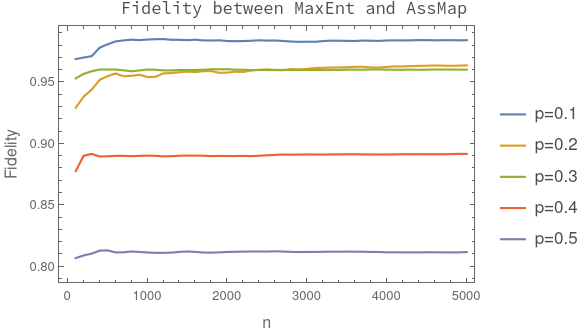
\includegraphics[width=0.6\linewidth]{general/figures/fidelityMaxEntAssMap_vs_n.png}
    \caption{Fidelidad entre el estado de máxima entropía y el estado asignado por promedio como función del número de estados usados en el promedio, para diferentes valores del parámetro $p$.}
    \label{fig:FidMaxEntAssMapN}
\end{figure}
La figura \ref{fig:FidMaxEntAssMapN} muestra que la fidelidad entre ambos estados parece constante siempre que $n>1000$, y que la verdadera dependencia se halla sobre el parámetro $p$. Veamos, pues, la fidelidad entre ambos estados como función de $p$, con $n=1000$.
\begin{figure}[h!]
    \centering
    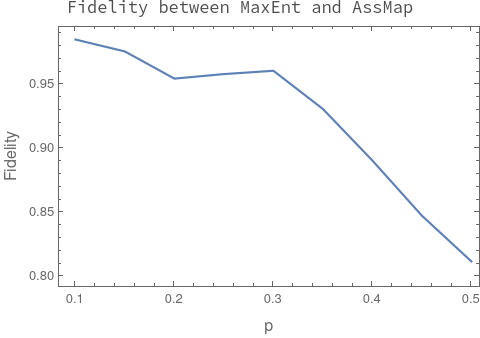
\includegraphics[width=0.6\linewidth]{general/figures/fidelityMaxEntAssMap_vs_p.png}
    \caption{Fidelidad entre el estado de máxima entropía y el estado asignado por promedio como función de $p$.}
    \label{fig:FidMaxEntAssMapP}
\end{figure}
La figura \ref{fig:FidMaxEntAssMapP} es algo burda, y puede que requiera más puntos y observaciones, pero parece revelar que los estados tienden a ser el mismo cuando $p\rightarrow 0,1$. Asumo aquí simetría respecto a $p=0.5$. \notaAd{Bastará con generar puntos entre 0.5 y 1}.
\newpage


\chapter{Resultados para el estado de máxima entropía}

\section{El estado de máxima entropía en términos de $r_{z}$}

La forma matricial de este estado es:
\begin{equation*}
\left(
\begin{array}{cccc}
 \frac{1}{4} e^{-\lambda_{3}} \text{sech}(\lambda_{3} p)
   \text{sech}(\lambda_{3}-\lambda_{3} p) & 0 & 0 & 0 \\
 0 & \frac{e^{2 \lambda_{3}}}{\left(e^{2 \lambda_{3}
   p}+1\right) \left(e^{2 \lambda_{3}}+e^{2 \lambda_{3}
   p}\right)} & 0 & 0 \\
 0 & 0 & \frac{1}{\left(e^{2 \lambda_{3}}+1\right) e^{-2
   \lambda_{3} p}+e^{2 \lambda_{3}-4 \lambda_{3}
   p}+1} & 0 \\
 0 & 0 & 0 & \frac{1}{4} e^{\lambda_{3}}
   \text{sech}(\lambda_{3} p) \text{sech}(\lambda_{3}-\lambda_{3} p) \\
\end{array}
\right)
\end{equation*}
Hallar el valor de $\lambda_{
3}$ en términos del valor $r_{z}$ implica resolver la ecuación:
\begin{equation}\label{eq:RZ}
rz=-\frac{1}{2}\frac{\sinh(\lambda_{3})+(1-2p)\sinh((1-2p)\lambda_{3})}{\cosh(p\lambda_{3})\cosh((1-p)\lambda_{3})}
\end{equation}
No se ve ninguna forma sencilla de despejar al multiplicador de Lagrange. En realidad, esto solo se puede si la función $r_{z}(\lambda_{3})$ tiene inversa, y esto puede depender del parámetro $p$. Graficar la superficie (Figura \ref{fig:rzsurf}) puede aclarar algo el panorama.
\begin{figure}[h!]
\centering
\begin{subfigure}{0.475\textwidth}
  \centering
  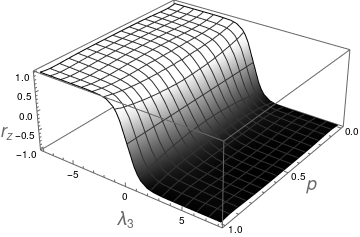
\includegraphics[width=0.6\linewidth]{maxent/figures/LagrangeMult_lambda-8to8.png}
  \caption{$-8<\lambda_{3}<8$}
\end{subfigure}%
\begin{subfigure}{0.475\textwidth}
  \centering
  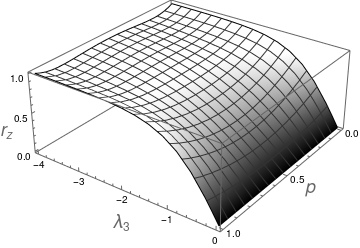
\includegraphics[width=0.6\linewidth]{maxent/figures/LagrangeMult_lambda-4to0.png}
  \caption{$-4<\lambda_{3}<0$}
\end{subfigure}
\caption{Superficie de $r_{z}$ según (\ref{eq:RZ}) para dos intervalos de $\lambda_{3}$. A valores $\lambda_{3}<0$ corresponden valores $r_{z}>0$ y viceversa.}
\label{fig:rzsurf}
\end{figure}

Después de una breve inspección se concluyen las siguientes cosas:
\begin{itemize}
\item la superficie es simétrica respecto al plano $p=0.5$
\item la superficie es antisimétrica  respecto al plano $\lambda_{3}=0$ i.e. $r_{z
}(\lambda_{3},p)=-r_{z
}(-´\lambda_{3},p)$
\item $\text{sgn}(\lambda_{3})=-\text{sgn}(r_{z})$
\end{itemize}

La simetría respecto al plano $p=0.5$ suguiere un cambio de variable $q=\abs{p-0.5}$. La ecuación (\ref{eq:RZ}) se reescribe como:
\begin{equation}\label{eq:RZq}
r_{z}=-\frac{1}{2}\frac{\sinh(\lambda_{3})+2q\sinh(2q\lambda_{3})}{\cosh((q+\frac{1}{2})\lambda_{3})\cosh((q-\frac{1}{2})\lambda_{3})}
\end{equation}
Y nos limitamos al dominio $\lambda_{3}\leq0$ y $0\leq q\leq\frac{1}{2}$. Podemos graficar la función (\ref{eq:RZq}) para diferentes valores de $q$ (Figura \ref{fig:rzinv}).
\begin{figure}[h!]
\centering
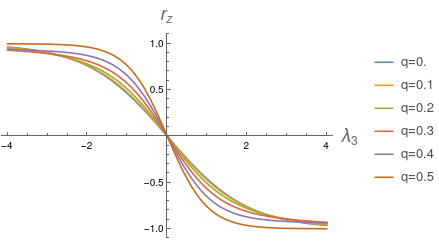
\includegraphics[width=0.6\linewidth]{maxent/figures/rz_has_inverse_lambda-4to4.png}
\caption{$r_{z}$ como función de $\lambda_{3}$ para diferentes valores de $q$. La apariencia uno a uno sugiere la existencia de una inversa.}
\label{fig:rzinv}
\end{figure}

\subsection{Dos soluciones particulares}

Considerando el caso $q=\frac{1}{2}$, la ecuación (\ref{eq:RZq}) se reduce a 
\begin{equation}
r_z=-\frac{1}{2}\frac{2\sinh(\lambda_{3})}{\cosh(\lambda_{3})}
\end{equation}
de manera que $\lambda_{3}=-\text{arctanh}(rz)$.

Si $q=0$, la ecuación (\ref{eq:RZq}) se reduce a
\begin{equation}
r_z=-\frac{\sinh(\lambda_{3})}{\cosh(\lambda_{3}+1)}
\end{equation}
Mathematica sugiere la solución:
\begin{equation}\label{eq:lambda0.5}
\lambda_{3}=\log\qty(\frac{1-r_{z}}{1+r_{z}}).
\end{equation}
\section{La dinámica analítica para el caso $\mcU=\textsc{SWAP}$}

Si se escribe $Z=\Tr{\exp(\lambda_{2}\hat{G}_{3})}$, el estado de máxima entropía compatible con $\rho$ es
\begin{equation}
\varrho_{max}=\frac{1}{Z}\begin{pmatrix}
 e^{-\lambda } & 0 & 0 & 0 \\
 0 & e^{-\lambda  (2 p-1)} & 0 & 0 \\
 0 & 0 & e^{\lambda  (2 p-1)} & 0 \\
 0 & 0 & 0 & e^{\lambda } \\
\end{pmatrix}.
\end{equation}
Este operador de densidad es separable. Es decir, tiene la forma $\varrho_{max}=\varrho_{max}^{A}\otimes\varrho_{max}^{B}$.

Si se aplica el mapeo de grano gureso a este estado, el resultado es precisamente, $\rho$. Si se deja esto en términos de $\lambda_{3}$:
\begin{equation}
\rho(0)=\CG{\varrho_{max}}=\frac{1}{Z}\begin{pmatrix}
 e^{-\lambda }+(1-p)e^{\lambda  (2 p-1)}+p e^{-\lambda  (2 p-1)} & 0 \\
 0 & e^{\lambda }+p e^{\lambda  (2 p-1)}+(1-p)e^{-\lambda  (2 p-1)} \\
\end{pmatrix}.
\end{equation}
El resultado de la dinámica efectiva se puede calcular de forma directa, y es
\begin{equation}
\rho(t=1)=\frac{1}{Z}\CG{S\varrho_{z} S}=
\begin{pmatrix}
 e^{-\lambda }+p e^{\lambda  (2 p-1)}+(1-p) e^{-\lambda  (2 p-1)} & 0 \\
 0 & e^{\lambda }+p e^{-\lambda  (2 p-1)}+(1-p)e^{\lambda  (2 p-1)} \\
\end{pmatrix}
\end{equation}

\subsection{Caso $p=\frac{1}{2}$}

Dentro del estado de máxima entropía, los exponentes de los elementos no extremos de la diagonal se anulan. El resultado es
\begin{equation}
\varrho_{max}=\frac{1}{Z}
\begin{pmatrix}
 e^{-\lambda } & 0 & 0 & 0 \\
 0 & 1. & 0 & 0 \\
 0 & 0 & 1. & 0 \\
 0 & 0 & 0 & e^{\lambda } \\
\end{pmatrix}.
\end{equation}
Usando este, se obtienen tanto el estado efectivo inicial como el estado efectivo final, ambos en términos del multiplicador de Lagrange, y son
\begin{align}
\rho(0)=\CG{\varrho_{max}}=\frac{1}{Z}
\begin{pmatrix}
 1.\, +e^{-\lambda } & 0 \\
 0 & 1.\, +e^{\lambda } \\
\end{pmatrix}, && \rho(1)=\CG{S\varrho_{max} S}=\frac{1}{Z}
\begin{pmatrix}
 1.\, +e^{-\lambda } & 0 \\
 0 & 1.\, +e^{\lambda } \\
\end{pmatrix}.
\end{align}
Si se usa (\ref{eq:lambda0.5}) se halla:
\begin{equation}
\varrho_{max}=\frac{1}{Z}
\begin{pmatrix}
 \frac{1}{4} \left(r_z+1\right){}^2 & 0 & 0 & 0 \\
 0 & \frac{1}{4} \left(1-r_z^2\right) & 0 & 0 \\
 0 & 0 & \frac{1}{4} \left(1-r_z^2\right) & 0 \\
 0 & 0 & 0 & \frac{1}{4} \left(r_z-1\right){}^2 \\
\end{pmatrix}.
\end{equation}
Y recuperamos los estados inicial y final esperados:
\begin{align}
\rho(0)=\CG{\varrho_{max}}=\frac{1}{Z}\begin{pmatrix}
 \frac{1}{2} \left(r_z+1\right) & 0 \\
 0 & \frac{1}{2} \left(1-r_z\right) \\
\end{pmatrix}, && \rho(1)=\frac{1}{Z}\CG{S\varrho_{max} S}=
\begin{pmatrix}
 \frac{1}{2} \left(r_z+1\right) & 0 \\
 0 & \frac{1}{2} \left(1-r_z\right) \\
\end{pmatrix}.
\end{align}

\newpage

\chapter{Resultados para el mapeo de asignación}

\section{Parte analítica}


\subsection{SWAP}
\subsubsection{Estado fino compatible arbitrario}
Sea $\rho\in\mcL(\mcH_{2})$ un estado grueso sobre z definido como en (\ref{eq:rhoz}) y $\varrho$ un estado fino compatible con parametrización de Bloch $\vec{\gamma}$. Sabemos que la acción del coarse graining sobre $\varrho$ es
\begin{equation}\label{eq:CGSWAPprei}
\CG{\varrho}=\frac{1}{2}\qty(\Id+\sum_{k=1}^{3}(p\gamma_{k,0}+(1-p)\gamma_{0,k})\sigma_{k}).
\end{equation}
Este estado, claro, debe estar alineado con el eje $z$, así que se cumple que $p\gamma_{k,0}+(1-p)\gamma_{0,k}=0$ para $k=1,2$. De esta forma, el estado queda como
\begin{equation}\label{eq:CGSWAPi}
\CG{\varrho}=\frac{1}{2}\qty(\Id+(p\gamma_{3,0}+(1-p)\gamma_{0,3})\sigma_{z}).
\end{equation}
Luego, si se aplica el SWAP, el estado grueso efectivo es
\begin{equation}\label{eq:CGSWAPfi}
\CG{S\varrho S}=\frac{1}{2}\qty(\Id+\sum_{k=1}^{3}(p\gamma_{0,k}+(1-p)\gamma_{k,0})\sigma_{k}).
\end{equation}
Para que las ecuaciones (\ref{eq:CGSWAPi}) y (\ref{eq:CGSWAPfi}) correspondan al mismo estado (esto es, que la dinámica efectiva sea la identidad), primero debe de cumplirse que $p\gamma_{0,k}+(1-p)\gamma_{k,0}=0$ para $k=1,2$. Si se combinan ambas condiciones sobre estas componentes se obtiene
\begin{align*}
(2p-1)(\gamma_{k,0}-\gamma_{0,k})&=0,\\
\gamma_{k,0}+\gamma_{0,k}&=0.
\end{align*}
Esto asegura que el estado descrito por (\ref{eq:CGSWAPfi}) esté sobre el eje z, pero para que la coordenada en dicho eje no cambie tras el SWAP subyacente debe cumplirse que 
\begin{equation*}
(2p-1)(\gamma_{3,0}-\gamma_{0,3})=0,
\end{equation*}
De esta forma, puede verse que un estado $\psi$ que cumpla que $\gamma_{k,0}=\gamma_{0,k}=0$ para $k=1,2$ y que $\gamma_{3,0}=\gamma_{0,3}$ no se ve afectado por el SWAP de forma efectiva. Esta invarianza es completamente dependiente del estado fino inicial (o del estado grueso inicial), y las condiciones sobre las componentes se cumplen \notaAd{solo si, estoy seguro de que si se revisan las constantes de estructura sí sale el solo si} si $\rho_{z}$ es puro, y por consiguiente $\varrho=\rho_{z}\otimes\rho_{z}$.

Además, la dinámica efectiva es la identidad siempre que $p=0.5$. Para dicho valor de $p$ se satisfacen todas las condiciones.

\subsubsection{Mapeo de asignación}

Sea $\{\varrho^{j}\}_{j=1}^{N}$ el conjunto usado en el mapeo de asignación, y $\{\vec{\gamma}^{j}\}_{j=1}^{N}$ el conjunto de sus parametrizaciones de Bloch. En tal caso los estados efectivos inicial y final son:
\begin{align}
\rho&=\frac{\sigma_{z}}{N}\sum_{j}(p\gamma_{3,0}^{j}+(1-p)\gamma_{0,3}^{j}),\\
\rho'&=\frac{\sigma_{z}}{N}\sum_{j}(p\gamma_{0,3}^{j}+(1-p)\gamma_{3,0}^{j}).
\end{align}
La dinámica efectiva vuelve a ser la identidad si $p=0.5$ o si $\rho_{z}$ es puro


\newpage


\section{Parte numérica}
\subsection{Cascarón de estados mixtos}
Se generan estados puros $\begin{pmatrix}
a\\
b\\ \end{pmatrix}$ de manera uniforme. Estos son puntos en el cascarón unitario. Todos estos puntos se deplazan radialmente hacia adentro mediante un factor:
\begin{equation}
\vec{\alpha}=r\vec{\alpha_{0}}
\end{equation}
El resultado es un conjunto de estados mixtos $\{\rho_{i}\}_{i=1}^{N}$ cuyos vectores de Bloch se encuentran en el cascarón de radio $r$.

\subsubsection{Mapeo de asignación para el cascarón}


A cada $\rho_{i}$ hay que hallarle su estado fino asignado. Lo que se hace es generar un conjunto $\{\psi_{i}\}_{i=1}^{N}$ de estados finos para un estado grueso en $z$, $\rho_{z}$, tal que su coordenada en $z$ es justamente el radio del cascarón.

Como existe una unitaria $U_{i}$ entre $\rho_{z}$ y cada estado de $\{\rho_{i}\}_{i=1}^{N}$. Entonces podemos aplicar estas unitarias para hallar todos los $\mcA[\rho_{i}]$.

\subsection{Resultados}

Dos experimentos. En el primero se utiliza una probabilidad de swap $p=0.5$ (cascarón de radio $r=0.3$). El conjunto no cambia. En el segundo se utiliza una probabilidad de swap $p=0.3$ (cascarón de radio $r=0.8$).

Se grafican dichos cascarones en azul. Se aplica un SWAP a todos los $\mcA[\rho_{i}]$, y se saca el coarse graining. El resultado se grafica en amarillo.

\begin{figure}[h]
\centering
\begin{subfigure}{0.4\textwidth}
  \centering
  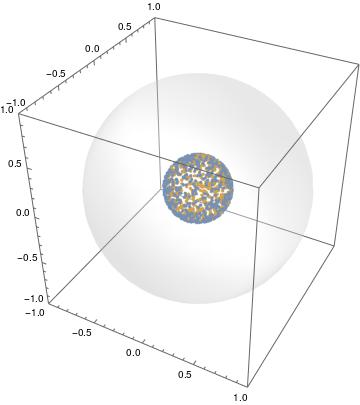
\includegraphics[width=0.8\linewidth]{assmap/figures/effectiveswap_p=0.5_z=0.3.jpeg}
  \caption{$p=0.5$, $r=0.3$, el conjunto no cambia después del swap subyacente}
  \label{fig:paralelogram}
\end{subfigure}
\begin{subfigure}{0.4\textwidth}
  \centering
  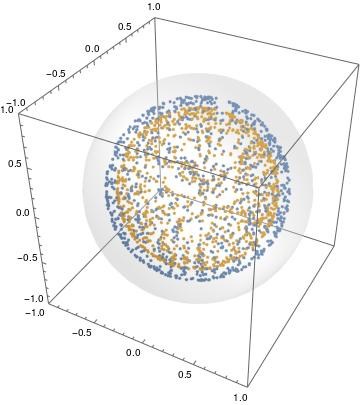
\includegraphics[width=0.8\linewidth]{assmap/figures/effectiveswap_p=0.3_z=0.8.jpeg}
  \caption{$p=0.5$, $r=0.3$, el conjunto se contrae  después del swap subyacente}
  \label{fig:paralelogram}
\end{subfigure}
\label{fig:cooldensities}
\end{figure}
\chapter{Dinámicas efectivas}
\section{La dinámica analítica para el caso $\mcU=\textsc{SWAP}$}
En esta sección se desarrollan resultados analíticos para una evolución unitaria subyacente descrita por el operador \textsc{SWAP}.

\subsection{Evolución de $t=0$ a $t=1$}

Utilizando la expresión (\ref{eq:MaxEntSeparable}), se puede pasar tanto a $\varrho_{max}(0)$ como a $\varrho_{max}(1)$ a través de la aplicación de grano grueso. El resultado $\CG{\varrho_{max}(0)}$ corresponde al estado grueso inicial, pero en términos de $\lambda$. Así:
\begin{equation}
\rho(0)=\frac{1}{2}[\Id+(\hat{r}_{\rho}\cdot\vec{\sigma})(p\tanh{\lambda p}+(1-p)\tanh{\lambda (1-p)})],
\end{equation}
\begin{equation}
\rho(t=1)=\frac{1}{2}[\Id+(\hat{r}_{\rho}\cdot\vec{\sigma})((1-p)\tanh{\lambda p}+p\tanh{\lambda (1-p)})].
\end{equation}
Vemos que ambos estados tienen la misma orientación pero pureza distinta. Esto significa que el efecto del \textsc{SWAP} subyacente sobre la esfera de Bloch es comprimir al estado efectivo inicial con un coeficiente $\kappa_{1}$ tal que
\begin{equation}\label{eq:SWAPFactor}
  \kappa_{1}=\frac{r_{\rho(1)}}{r_{\rho(0)}}=\frac{(1-p)\tanh{\lambda p}+p\tanh{\lambda (1-p)}}{
    p\tanh{\lambda p}+(1-p)\tanh{\lambda (1-p)}}
\end{equation}
Claro está, el factor de compresión depende del multiplicador de Lagrange, que a su vez es una función de la pureza del estado inicial. La figura \ref{fig:SWAPFactor2D} muestra dicha dependencia. Si la dependencia del factor de compresión en el estado efectivo inicial se denota por un superíndice, la dinámica efectiva puede escribirse como
\begin{equation}\label{eq:EffectiveSWAP1}
  \boxed{\frac{1}{2}(\Id+\vec{r}_{\rho}\cdot\vec{\sigma}) \xrightarrow{S} \frac{1}{2}(\Id+\kappa_{1}^{\rho}\vec{r}_{\rho}\cdot\vec{\sigma})}
\end{equation}
De las ecuaciónes (\ref{eq:SWAPFactor}) y (\ref{eq:EffectiveSWAP1}) distinguimos lo siguiente:
\begin{itemize}
  \item Si $p=0.5$, entonces $\kappa_{1}^{\rho}=1$. Esto se debe a que la aplicación borrosa es invariante bajo el $\textsc{SWAP}$ si $p=0.5$.
  \item $\kappa_{1}^{\rho}$ no depende de la orientación del vector de Bloch, únicamente depende de la magnitud $r_{\rho(0)}$ y $p$.
  \item En los casos extremos, $p=1$ o $p=0$, la esfera colapsa al origen.
\end{itemize}

\begin{figure}[h!]
  \centering
  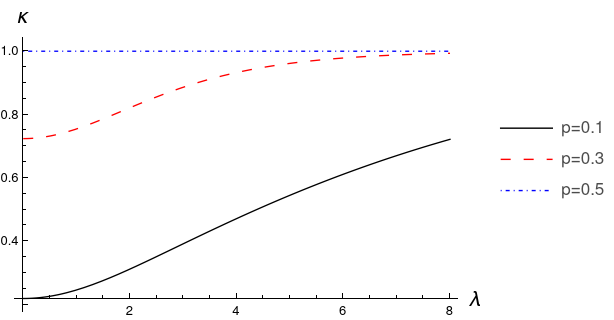
\includegraphics[width=0.6\linewidth]{maxent/figures/ContractionFactorSWAP_2D_lambda0to8.png}
  \caption{Factor de compresión $\kappa_{1}$ como función de $\lambda$, para diferentes valores de $p$.}
  \label{fig:SWAPFactor2D}
\end{figure}

Como el factor de compresión depende de $\lambda$, la dinámica no es lineal. Las operaciones cuánticas de un qubit se traducen como aplicaciones afines en la esfera de Bloch. Si quisiéramos ver el proceso asociado al \textsc{SWAP} subyacente como una transformación de la forma
\begin{equation*}
  \vec{r}\rightarrow M\vec{r}+\vec{c}
\end{equation*}
en la que $\vec{c}=0$, y $M=OS$ con $O=\Id$ y $S=\kappa_{1}(\vec{r})\Id$, de tal forma que
\begin{equation*}
  \vec{r}\rightarrow \kappa_{1}(\vec{r})\vec{r}
\end{equation*}
nos daríamos cuenta que la transformación no es afín, y por esto, el proceso no puede ser descrito a través del formalismo de las operaciones cuánticas (no tiene representación en operadores de Kraus) \cite{Chuang}.
  \begin{figure}[h!]
    \centering
    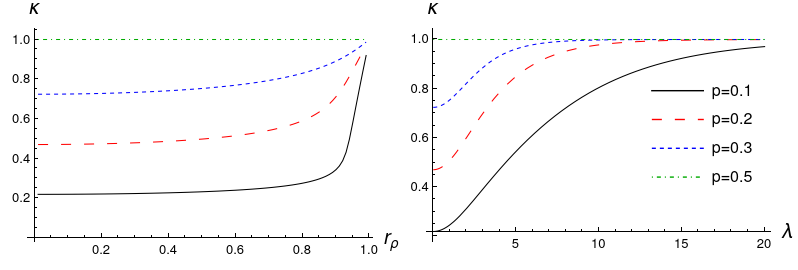
\includegraphics[width=0.9\linewidth]{maxent/figures/ContractionFactorSWAP_2D_both.png}
    \caption{Factor de compresión $\kappa_{1}$ como función de $r_{\rho}$ (der.) y como función de $\lambda$ (izq.), para diferentes valores de $p$.}
    \label{fig:SWAPFactor2Drl}
  \end{figure}
\subsubsection{Caso $p=\frac{1}{2}$}

Aunque es posible repetir todas las cuentas desde la contrucción del estado de máxima entropía, haciendo $p=\frac{1}{2}$, basta con ver que el factor (\eqref{eq:SWAPFactor}) es $1$ en dicho caso. Así, todos los estado gruesos son puntos fijos bajo una evolución subyacente SWAP con aplicación de grano grueso con parámetro $p=\frac{1}{2}$.

\subsection{Extensión a $t$}
Siendo \textsc{SWAP} un operador unitario, anteriormente se denotó el estado inicial y final como $\varrho(0)$ y $\varrho(1)$, de acuerdo a lo establecido en la ecuación (\ref{eq:TimeDepenenceUnitary}). Para extender los resultados a un tiempo arbitrario en el intervalo $[0,1]$, es necesaria una expresión analítica del operador. El operador SWAP deja intactos a los estados $\ket{00}$ y $\ket{11}$, e intercambia $\ket{01}$ con $\ket{1,0}$. De esto, el operador también dejará invariantes (hasta un factor) a los estados $\ket{+_{2}}=\frac{\ket{01}+\ket{10}}{\sqrt{2}}$ y $\ket{-_{2}}\frac{\ket{01}-\ket{10}}{\sqrt{2}}$. Dados estos eigenestados (y eigenvalores), la descomposición espectral del operador es
\begin{equation}\label{eq:SWAPSpectral}
S=P(\dyad{00}+\dyad{11}+\dyad{+_{2}}-\dyad{-_{2}})P^{\dag}.
\end{equation}
donde $P$ es la matriz formada por los eigenestados del operador. Potenciando se halla que
\begin{align}\label{eq:SWAPPower}
S^{t}&=P(\dyad{00}+\dyad{11}+\dyad{+_{2}}+(-)^{t}\dyad{-_{2}})P^{\dag}\\
&=P(\dyad{00}+\dyad{11}+\dyad{+_{2}}+e^{i \pi t}\dyad{-_{2}})P^{\dag}
\end{align}
La forma matricial del operador \textsc{SWAP} a un tiempo $t$ es
\begin{equation}
S^{t}=\begin{pmatrix}
 1 & 0 & 0 & 0 \\
 0 & \frac{1}{2}(1+e^{i \pi t}) & \frac{1}{2} (1-e^{i \pi t}) & 0 \\
 0 & \frac{1}{2}(1-e^{i \pi t}) & \frac{1}{2}(1+e^{i \pi t}) & 0 \\
 0 & 0 & 0 & 1
\end{pmatrix}=\begin{pmatrix}
  1 & 0 & 0 & 0 \\
  0 & e^{i\frac{t\pi}{2}}\cos{\frac{t\pi}{2}} & -ie^{i\frac{t\pi}{2}}\sin{\frac{t\pi}{2}} & 0 \\
  0 & -ie^{i\frac{t\pi}{2}}\sin{\frac{t\pi}{2}} & e^{i\frac{t\pi}{2}}\cos{\frac{t\pi}{2}}  & 0 \\
  0 & 0 & 0 & 1
 \end{pmatrix}
\end{equation}
Con ayuda de Mathematica pude aplicar este operador para obtener que
\begin{equation}
  \rho(t)=\frac{1}{2}\{\Id+(\hat{r_{\rho}}\cdot\vec{\sigma})[((1-p)\cos^{2}{\frac{\pi t}{2}}+p\sin^{2}{\frac{\pi t}{2}})\tanh{p\lambda}+(p\cos^{2}{\frac{\pi t}{2}}+(1-p)\sin^{2}{\frac{\pi t}{2}})\tanh{(1-p)\lambda}]\}.
\end{equation}
De esto, el factor de compresión dependiente del tiempo es
\begin{equation}\label{eq:SWAPFactort}
  \kappa_{t}^{\rho}=\frac{(p\cos^{2}{\frac{\pi t}{2}}+(1-p)\sin^{2}{\frac{\pi t}{2}})\tanh{\lambda p}+((1-p)\cos^{2}{\frac{\pi t}{2}}+p\sin^{2}{\frac{\pi t}{2}})\tanh{\lambda (1-p)}}{
    p\tanh{\lambda p}+(1-p)\tanh{\lambda (1-p)}}
\end{equation}

\begin{figure}[h!]
  \centering
  \begin{subfigure}{0.32\textwidth}
    \centering
    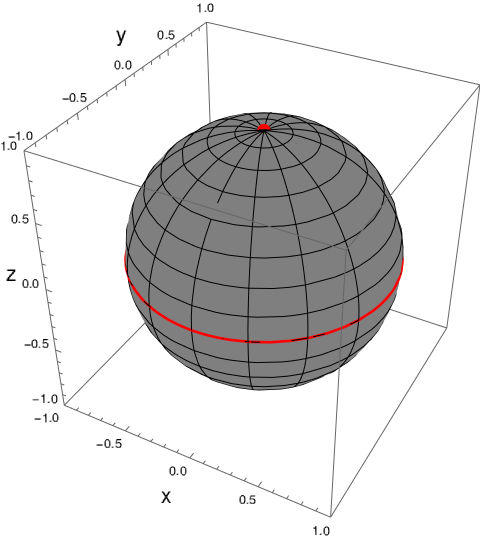
\includegraphics[width=0.9\linewidth]{maxent/figures/sphere_swapcontraction_t=0.0_z=0.9_p=0.9.png}
    \caption{$t=0$}
  \end{subfigure}%
  \begin{subfigure}{0.32\textwidth}
    \centering
    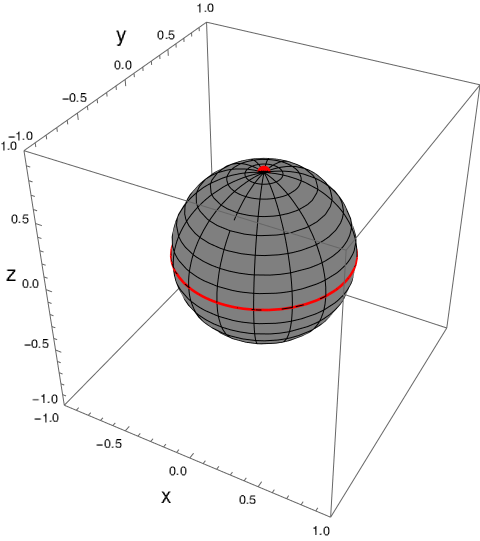
\includegraphics[width=0.9\linewidth]{maxent/figures/sphere_swapcontraction_t=0.5_z=0.9_p=0.9.png}
    \caption{$t=0.5$}
  \end{subfigure}
  \begin{subfigure}{0.32\textwidth}
    \centering
    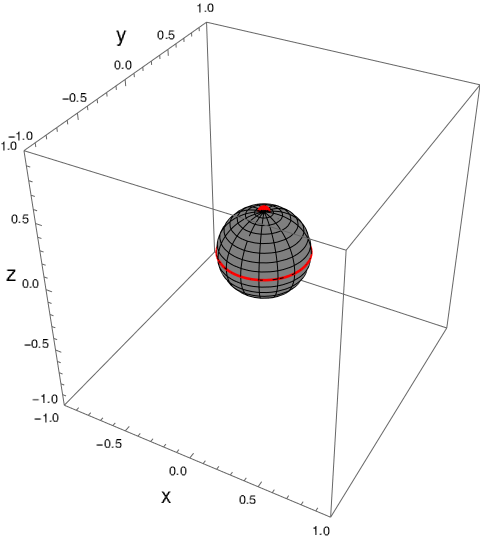
\includegraphics[width=0.9\linewidth]{maxent/figures/sphere_swapcontraction_t=1.0_z=0.9_p=0.9.png}
    \caption{$t=1$}
  \end{subfigure}
  \caption{Efecto de la evolución subyacente si $r_{z}=0.9$, $p=0.9$. La dramática contracción se asocia a una pérdida casi total de información.}
  \label{fig:SWAPFactorSequence}
  \end{figure}
En términos del valor esperado del observable $\sigma_{z}$, la evolución del estado se da como
\begin{equation}
  \expval{\sigma_{z}(t)}=\kappa_{t}^{\rho}\expval{\sigma_{z}(0)}
\end{equation}
que puede escribirse, también, como las probabilidades de que $\rho(t)$ se halle en el estado $\ket{0}$ o $\ket{1}$
 \begin{align}
  \bra{0}\rho(t)\ket{0}=\frac{1}{2}(1+\kappa_{t}^{\rho}\expval{\sigma_{z}(0)}) && \bra{1}\rho(t)\ket{1}=\frac{1}{2}(1-\kappa_{t}^{\rho}\expval{\sigma_{z}(0)}
 \end{align}
 donde la dependencia temporal está completamente contenida dentro del factor $\kappa_{t}^{\rho}$. 
\newpage
\section{La dinámica para la compuerta controlled-not}
La compuerta \textit{controlled not}, o CNOT, es el análogo cuántico de la compuerta lógica XOR. La compuerta XOR recibe como entrada dos bits, y arroja uno que puede ser $0$ si los bits de entrada tienen el mismo valor, o $1$ si tienen valores diferentes. Por otro lado, la compuerta cuántica CNOT actúa sobre un sistema de dos qubits, aplicando sobre el segundo qubit la compuerta $\sigma_{1}$ (NOT) si el primer qubit se halla en el estado $\ket{1}$, o dejándolo invariante si el primer qubit se halla en el estado $\ket{0}$. Esto es, cumple que \cite{Chuang}
\begin{align*}
    \ket{0}\otimes\ket{0}\mapsto\ket{0}\otimes\ket{0}\\
    \ket{0}\otimes\ket{1}\mapsto\ket{0}\otimes\ket{1}\\
    \ket{1}\otimes\ket{0}\mapsto\ket{1}\otimes\ket{1}\\
    \ket{1}\otimes\ket{1}\mapsto\ket{1}\otimes\ket{0} \rlap{.}
\end{align*}
En la base de los eigenestados de $\pauli{3}\otimes\pauli{3}$, la compuerta puede representarse como la matriz de permutación
\begin{equation*}
    \cnot=\begin{pmatrix}
        1&0&0&0\\
        0&1&0&0\\
        0&0&0&1\\
        0&0&1&0
    \end{pmatrix}.
\end{equation*}

Claro está, esta matriz corresponde a la evolución discreta. Para hallar la extensión a cualquier tiempo $t$, notamos que los eigenestados de este operador son $\ket{01}$, $\ket{00}$, $\ket{+}_{\cnot}$ y $\ket{-}_{\cnot}$ donde se definen
\begin{align*}
  \ket{+}_{\cnot}=\frac{\ket{10}+\ket{11}}{\sqrt{2}} & & \text{y} & & \ket{-}_{\cnot}=\frac{\ket{10}-\ket{11}}{\sqrt{2}}.
\end{align*}
Con esto es posible escribir la descomposición espectral del operador, y luego potenciarla 
\begin{align*}
\cnot=&P(\dyad{00}+\dyad{01}+\dyad{+}_{\cnot}-\dyad{-}_{\cnot})P^{\dag}\\
\Rightarrow \cnot^{t}=&P(\dyad{00}+\dyad{11}+\dyad{+}_{\cnot}+e^{i \pi t}\dyad{-}_{\cnot})P^{\dag}.
\end{align*}
La forma matricial del operador controlled not a un tiempo $t$ es análoga a la del operador SWAP:
\begin{equation}\label{eq:CNOT(t)}
\cnot^{t}=\begin{pmatrix}
  1 & 0 & 0 & 0 \\
  0 & 1 & 0 & 0 \\
  0 & 0 & e^{i\frac{t\pi}{2}}\cos{\frac{t\pi}{2}} & -ie^{i\frac{t\pi}{2}}\sin{\frac{t\pi}{2}}\\
  0 & 0 & -ie^{i\frac{t\pi}{2}}\sin{\frac{t\pi}{2}} & e^{i\frac{t\pi}{2}}\cos{\frac{t\pi}{2}}
 \end{pmatrix}
\end{equation}
Y esta es la cosa: esta definición del operador CNOT está bien, pero es muy arbitraria. Si trabajamos en la base de los eigenestados de $\pauli{1}$, CNOT también puede verse como un operador que voltea al qubit de control si el qubit objetivo está en el estado $\ket{+}$. Aún más lo de \textit{negar} qubits realmente solo tiene sentido cuando estos son puros y cuando se hallan en estados completamente alineados con el eje $z$ (si trabajamos en la base de $\pauli{3}$) o con el eje $x$ (si trabajamos en la base de $\pauli{1}$). En realidad, CNOT puede verse como una operación que induce un entrelazamiento entre las partículas siempre que el qubit de control no se halla completamente alineado con el eje $z$. La descripción del operador CNOT a través de una tabla de verdad es apegarse de forma innecesaria al paradigma del cómputo clásico. De ahí que me halla costado tanto trabajo trabajar con este operador.

El operador \textsc{CNOT} puede expandirse de la siguiente manera:
\begin{equation*}
        \cnot=\frac{1}{2}(\Id+\pauli{3}\otimes\Id+\Id\otimes\pauli{1}-\pauli{3}\otimes\pauli{1}).
\end{equation*}
Si se calcula el logaritmo de la compuerta es posible hallar el hamiltoniano generador de la unitaria,
\begin{equation*}
    H_{\cnot}=\frac{\pi}{4}\qty(\Id-\pauli{3}\otimes\Id-\Id\otimes\pauli{1}+\pauli{3}\otimes\pauli{1}),
\end{equation*}
que por ser una suma de operadores que conmutan entre sí, nos permite ver al controlled not como una aplicación consecutiva de tres unitarias diferentes
\begin{align*}
    \cnot&=e^{-i\frac{\pi}{4}\Id}e^{i\frac{\pi}{4}\pauli{3}\otimes\Id}e^{i\frac{\pi}{4}\Id\otimes\pauli{1}}e^{-i\frac{\pi}{4}\pauli{3}\otimes\pauli{1}}\\
    &=e^{-i\frac{\pi}{4}} (e^{i\frac{\pi}{4}\pauli{3}}\otimes \Id) (\Id \otimes e^{i\frac{\pi}{4}\pauli{1}}) e^{-i\frac{\pi}{4}\pauli{3}\otimes\pauli{1}}.
\end{align*}
Cuando se le expande en términos de productos tensoriales de operadores de Pauli, deja de ser claro el efecto clásico del CNOT, pero yo diría que esta es una mejor representación, porque está a un paso de expresarse en términos de compuertas de rotación y una de acoplamiento de Ising.
\subsection{CNOT completo efectivo}

Considérese el caso en que el aparato de medición no tiene un error asociado ($p=1$). En dicho caso, a través del principio de máxima entropía, se esperaría que el estado efectivo final fuera
\begin{equation*}
  \rho(t=1)=\rho(0)+\pauli{3}\rho(0)\pauli{3}=\frac{1}{2}(\Id+r_{3}\pauli{3}).
\end{equation*}


Este resultado viene del hecho que, en el caso $p=1$, el estado de máxima entropía es simplemente $\rho\otimes\frac{1}{2}$. ¿Por qué? Pues bien, con la interpretación de que CNOT aplica una compuerta $\pauli{3}$ sobre el qubit de control dependiendo del estado del qubit objetivo en la base de $\pauli{3}$, entonces se vuelve claro que si dicho qubit se halla en un estado completamente mezclado, el resultado será dicha mezcla: la mitad del tiempo se aplicará la compuerta, y la otra mitad, no (esto, claro está, cuando se toma la traza parcial, que ignora un montón de correlaciones y entrelazamientos que se forman durante el proceso).


Si se conociera la preparación microscópica del estado inicial, $\varrho$, el resultado de aplicar la compuerta de controlled not seguido de trazar al segundo sistema sería
\begin{equation*}
  \rho(t=1)=\frac{1}{2}\qty[\Tr_{1}(\varrho)+\pauli{3}\Tr_{1}(\varrho)\pauli{3}+\Tr(\pauli{1}\Tr_{2}(\varrho))(\Tr_{1}(\varrho)-\pauli{3}\Tr_{1}(\varrho)\pauli{3})]
\end{equation*}

Tanta traza marea, pero puede ser más claro si asumimos que al tiempo $t=0$ el sistema se halla en un estado separable $\varrho=\rho_{1}\otimes\rho_{2}$. En dicho caso es claro que la evolución está induciendo correlaciones entre ambos sistemas (correlaciones visibles únicamente en las compontentes $x$ e $y$ del primer subsistema), y que dicha correlación depende completamente de $\Tr(\sigma_{1}\rho_{2})$ (el valor esperado de la componente en $x$ del segundo susbsistema). De nuevo, como trazamos al segundo sistema, es más importante ver a este como el sistema de control, del que depende la acción sobre el sistema que nos interesa.

Para estudiar la dinámica efectiva del operador $\cnot$ son particularmente útiles las expresiones (\ref{eq:rhoArhoB}). Como el estado de máxima entropía compatible con la aplicación de grano grueso puede escribirse como $\varrho_{\max}=\rho_{A}\otimes\rho_{B}$, entonces hallar el estado efectivo final es un problema de álgebra, en efecto,
\begin{align*}
    \rho(t=1)=\frac{1}{2}[&p(\rho(0)+\sigma_{3}\rho_{A}\sigma_{3}+\Tr{\sigma_{1}\rho_{B}}[\rho_{A}-\sigma_{3}\rho_{A}\sigma_{3}])\\
    &+(1-p)(\rho(0)+\sigma_{1}\rho_{B}\sigma_{1}+\Tr{\sigma_{3}\rho_{A}}[\rho_{B}-\sigma_{1}\rho_{B}\sigma_{1}])].
\end{align*}
La estructura del estado final es una consecuencia directa de la aplicación borrosa. El primer término es el que vimos previamente, y el segundo es exactamente los mismo, pero para el que se han invertido los roles: es ahora el sistema que no nos interesa el que experimenta la acción del sistema de control.

En términos del vector de Bloch, que es una forma rápida de obtener el cambio de los observables y de la esfera, la dinámica se ve como
\begin{equation*}
    \vec{r}_{\rho}=(pr_{A}+(1-p)r_{B})\hat{r}_{\rho}\mapsto\begin{pmatrix}
        r_{B}(pr_{A}(\hat{r}_{\rho,1})^2+(1-p)\hat{r}_{\rho,1})\\
        r_{B}r_{A}(p\hat{r}_{\rho,1}\hat{r}_{\rho,2}+(1-p)\hat{r}_{\rho,2}\hat{r}_{\rho,3})\\
        r_{A}(p\hat{r}_{\rho,3}+(1-p)r_{A}(\hat{r}_{\rho,3})^{2})
    \end{pmatrix}.
  \end{equation*}
Lo que se observa es que las componentes $x$ e $y$ tienden a cero conforme $p$ tiende a uno. Las correlaciones que se generan sobre dichas componentes con un estado completamente mezclado se pierden (bajo la estimación de máxima entropía).

\subsection{CNOT efectivo a un tiempo arbitrario}

El CNOT efectivo a un tiempo arbitrario no me parece particularmente interesante, ahora que lo pienso. Pero puedo obtenerla sin mayor   problema. Ya tengo la expresión del CNOT para tiempos arbitrarios, después de todo.


  \begin{figure}[h!]
    \centering
    \begin{subfigure}{0.45\textwidth}
      \centering
      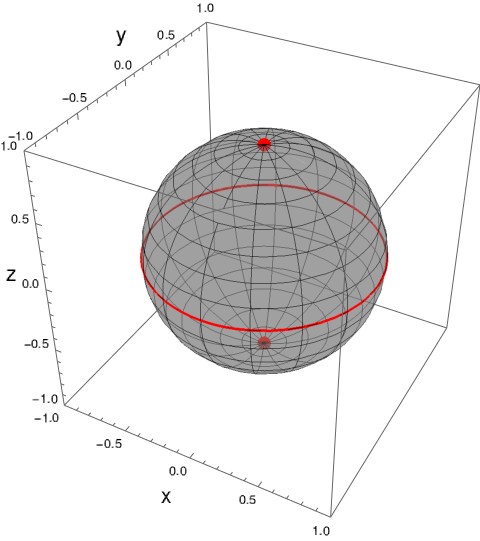
\includegraphics[width=0.9\linewidth]{maxent/figures/sphere_CNOT_t=0.0_z=0.8_p=0.95.png}
      \caption{$t=0$}
    \end{subfigure}%
    \begin{subfigure}{0.45\textwidth}
      \centering
      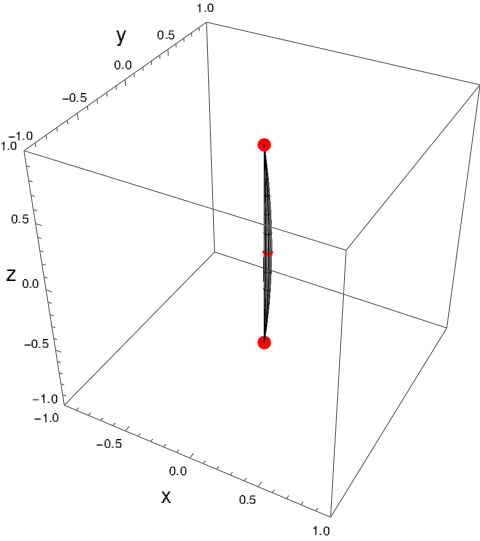
\includegraphics[width=0.9\linewidth]{maxent/figures/sphere_CNOT_t=1.0_z=0.8_p=0.95.png}
      \caption{$t=1.0$}
    \end{subfigure}
    \caption{Efecto de la evolución subyacente si $r=0.8$, $p=0.95$.}
    \label{fig:CNOTsequence2}
\end{figure}

\begin{figure}[h!]
    \centering
    \begin{subfigure}{0.45\textwidth}
      \centering
      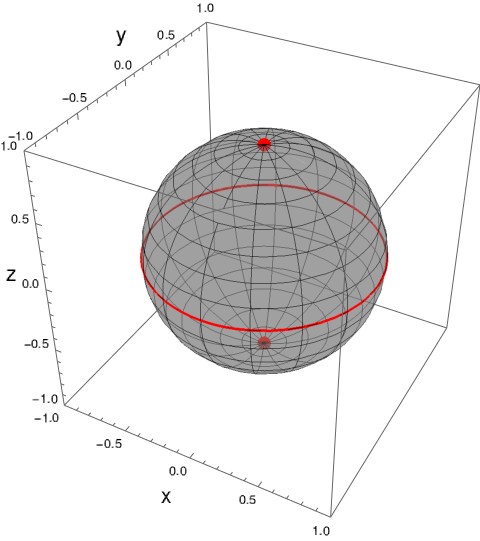
\includegraphics[width=0.9\linewidth]{maxent/figures/sphere_CNOT_t=0.0_z=0.8_p=0.6.png}
      \caption{$t=0$}
    \end{subfigure}%
    \begin{subfigure}{0.45\textwidth}
      \centering
      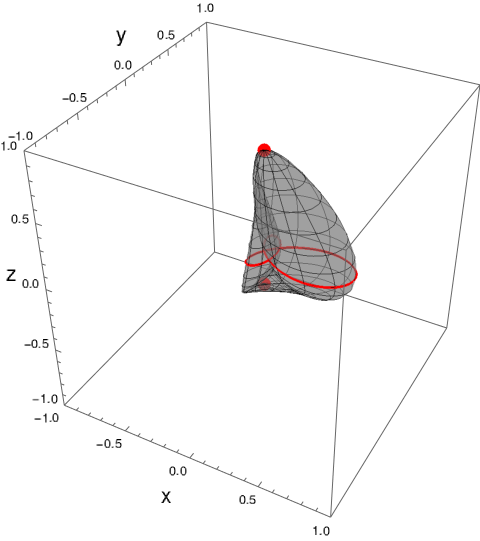
\includegraphics[width=0.9\linewidth]{maxent/figures/sphere_CNOT_t=1.0_z=0.8_p=0.6.png}
      \caption{$t=1.0$}
    \end{subfigure}
    \caption{Efecto de la evolución subyacente si $r=0.8$, $p=0.6$.}
    \label{fig:CNOTsequence2}
\end{figure}
\section{Evolución unitaria separable $\mcU=U_{1}\otimes U_{2}$}

Consideramos una unitaria $\mcU=U_{1}\otimes U_{2}$ que evoluciona en el tiempo como $\mcU_{t}=(U_{1}\otimes U_{2})^{t}=U_{1}^{t}\otimes U_{2}^{t}$. Retomando la ecuación (\ref{eq:MaxEntSeparable}), el estado efectivo evolucionado, en términos de un multiplicador de Lagrange y la unitaria $V$ que lo relaciona a un estado alineado en $z$ con la misma pureza es
\begin{align*}
    \CG{(U_{1}^{t}\otimes U_{2}^{t})\varrho_{max}(U_{1}^{t}\otimes U_{2}^{t})^{\dag}}&=p\frac{1}{Z_{1}}U_{1}^{t}V e^{\lambda p \sigma_{z}}V^{\dag}(U_{1}^t)^{\dag}+(1-p)\frac{1}{Z_{2}}U_{2}^{t}Ve^{\lambda (1-p)\sigma_{z}}V^{\dag}(U_{2}^t)^{\dag}\\
    &=p\frac{1}{Z_{1}}U_{1}^{t}V e^{\lambda p \sigma_{z}}(U_{1}^tV)^{\dag}+(1-p)\frac{1}{Z_{2}}U_{2}^{t}Ve^{\lambda (1-p)\sigma_{z}}(U_{2}^tV)^{\dag}\\
\end{align*}
Por un lado, podemos dejar a las unitarias $V$ dentro de las exponenciales, de tal forma que:
\begin{equation}
    \CG{(U_{1}^{t}\otimes U_{2}^{t})\varrho_{max}(U_{1}^{t}\otimes U_{2}^{t})^{\dag}}=p\frac{1}{2}(\Id+U_{1}^{t}(\hat{r}_{\rho}\cdot\vec{\sigma})(U_{1}^{t})^{\dag}\tanh{(\lambda p)})+(1-p)\frac{1}{2}(\Id+U_{2}^{t}(\hat{r}_{\rho}\cdot\vec{\sigma})(U_{2}^{t})^{\dag}\tanh{(\lambda (1-p))}).
\end{equation}
El resultado puede verse como las partes que componen al estado efectivo alineado en $z$ evolucionados por una composición de unitarias, que es otra unitaria. Las unitarias $U_{j}$ pueden escribirse como $e^{-i\theta_{j} \hat{n}_{j}\cdot\vec{\sigma}}$, mientras que $V=e^{i\alpha\hat{l}\cdot\vec{\sigma}}$ con $\hat{l}=(\cos{\beta},\sin{\beta},0)$, luego $U_{i}V=e^{i\zeta_{j} \hat{k}_{j}\cdot \vec{\sigma}}$ donde:
\begin{align*}
    \cos{\zeta_{j} }&=\cos{\theta_{j}}\cos{\alpha}-\hat{n}_{j}\cdot \hat{l}\sin{\theta_{j}}\sin{\alpha}\\
    \hat{k}_{j} &=\frac{1}{\sin{\zeta}}(\hat{n}_{j}\sin{\theta_{j}}\cos{\alpha}+\hat{l}\cos{\theta_{j}}\sin{\alpha}-\hat{n}_{j}\times \hat{l}\sin{\theta_{j}}\sin{\alpha})
\end{align*}
Total que la dinámica se ve como
\begin{equation}
    \boxed{V\CG{\varrho_{max}^{z}}V^{\dag} \xrightarrow{\mcU=U_{1}\otimes U_{2}} pW_{1}\Tr_{2}(\varrho_{max}^{z})W_{1}^{\dag}+(1-p)W_{2}\Tr_{1}(\varrho_{max}^{z})W_{2}^{\dag}}.
\end{equation}
Donde $W_{j}=U_{j}V$. Cada parte del estado efectivo se ve rotado de manera diferente. Las partes que se rotan son las partes que surgen al pasar al estado de máxima entropía por la aplicación de grano grueso. Pensando en esto, \notaAd{Regresar a la parte correspondiente: \ref{sec:CG(MaxEnt)}}. Aunque a mi me gusta la forma
\begin{equation}\label{eq:SeparableDynamics}
    \boxed{\rho\xrightarrow{\mcU=U_{1}\otimes U_{2}} p\frac{1}{Z_{1}}U_{1}e^{\lambda_{3}p\hat{r}_{\rho}\cdot\vec{\sigma}}U_{1}^{\dag}+(1-p)\frac{1}{Z_{2}}U_{2}e^{\lambda_{3}(1-p)\hat{r}_{\rho}\cdot\vec{\sigma}}U_{2}^{\dag}}.
\end{equation}

Si el estado inicial tiene componente en $z$ nomás
\begin{equation}\label{eq:SeparableZDynamics}
\CG{(U_{1}^{t}\otimes U_{2}^{t})\varrho_{max}(U_{1}^{t}\otimes U_{2}^{t})^{\dag}}=p\frac{1}{Z_{1}}e^{\lambda p U_{1}^{t}\sigma_{z}(U_{1}^t)^{\dag}}+(1-p)\frac{1}{Z_{2}}e^{\lambda (1-p)U_{2}^{t}\sigma_{z}(U_{2}^t)^{\dag}}
\end{equation}
Incluyendo el tiempo y haciendo el cambio $t\theta\rightarrow t$, los exponentes dentro de (\ref{eq:SeparableDynamics}) se desarrollan como:
\begin{align*}
    e^{-i\theta \hat{n}\cdot\vec{\sigma}}\sigma_{z}e^{i\theta \hat{n}\cdot\vec{\sigma}}&=(\Id\cos{t}-i\hat{n}\cdot\vec{\sigma}\sin{t})\sigma_{z}(\Id\cos{t}+i\hat{n}\cdot\vec{\sigma}\sin{t})\\
    &=\sigma_{z}\cos^{2}{t}+i[\sigma_{z},\hat{n}\cdot\vec{\sigma}]\sin{t}\cos{t}+(\hat{n}\cdot\vec{\sigma})\sigma_{z}(\hat{n}\cdot\vec{\sigma})\sin^{2}{t}\\
    &=\sigma_{z}+2\sin{t}\qty((n_{x}\sigma_{y}-n_{y}\sigma_{x})\cos{t}+n_{z}(\hat{n}\cdot\vec{\sigma})\sin{t})
\end{align*}
A notar que si $t=0$ no hay evolución. Luego, en el límite $t\ll 1$:
\begin{equation*}
    e^{-i\theta \hat{n}\cdot\vec{\sigma}}\sigma_{z}e^{i\theta \hat{n}\cdot\vec{\sigma}}=\sigma_{z}+2t(n_{x}\sigma_{y}-n_{y}\sigma_{x})
\end{equation*}
\notaAd{Aún tengo que darle interpretación a esto. Si defino $T=\theta^{-1}$ entonces este límite corresponde justamente a $T$ alta. Mañana voy a desarrollar esto como exponencial real de un vector de Pauli. La expresión es la misma que para la exponencial compleja, pero sin unidad imaginaria e intercambiano las funciones trigonométricas por hiperbólicas}

\subsection{El caso $U_{1}=\Id$ o $U_{2}=\Id$}
Retomando a expresión (\ref{eq:SeparableDynamics}), y en virtud de (\ref{eq:PauliVectorExp}), vemos que el estado efectivo inicial $\rho$ puede verse como una combinación de dos operadores con vector de Bloch con dirección $\hat{r}_{\rho}$. El vector de Bloch de $\rho$ se ve modificado al ser una de sus dos componentes (paralelas) rotada. La rotación siendo $U_{1}$ \notaAd{Creo que dependo mucho de las parametrizaciones de Bloch para entender lo que está pasadno, ¿qué sucede en el espacio de operadores de densidad?}. En general:
\begin{equation}\label{eq:SeparableDynamicsUxI}
    \rho\xrightarrow{\mcU=U_{1}\otimes \Id} p\frac{1}{Z_{1}}U_{1}e^{\lambda p\hat{r}_{\rho}\cdot\vec{\sigma}}U_{1}^{\dag}+(1-p)\frac{1}{Z_{2}}e^{\lambda(1-p)\hat{r}_{\rho}\cdot\vec{\sigma}}
\end{equation}
En términos del vector de Bloch, denotando $r_{A}=p\tan(p\lambda)$, $r_{B}=(1-p)\tan((1-p)\lambda)$, y $O$ la rotación generada por $U_{1}$:
\begin{equation}
    r\hat{r}_{\rho}\xrightarrow{\mcU=U_{1}\otimes \Id}r_{A}O\hat{r}_{\rho}+r_{B}\hat{r}_{\rho}=O(r\hat{r}_{\rho}-r_{B}\hat{r}_{\rho})+r_{B}\hat{r}_{\rho}
\end{equation}\label{eq:SeparableDynamicsUxIBloch}
El resultado es una rotación alrededor de una línea que no pasa por el origen. Una rotación de esta naturaleza puede descomponerse en una rotación a través de un eje que pasa por el origen $R$ y una traslación $T$ como $T^{-1}\circ R\circ T$. Notar que una transformación así no tendría por qué mantener a los estados dentro de la esfera de Bloch, por lo que esta debe depender del estado mismo. En efecto traslación tiene una magnitud $r_{B}$ en la dirección opuesta a la del estado (depende del estado tanto en magnitud como en dirección). Así que, aunque esto podría parecer una transformación afín, no lo es, pues depende enteramente del estado.

De (\ref{eq:SeparableDynamicsUxIBloch}) también se ve que si $U=e^{it\hat{n}\cdot\vec{\sigma}}$ entonces se ve que cualquier estado con vector de Bloch $r\hat{n}$ será invariante bajo la transformación subyacente. Lo que es mejor, esto aplica para cualquiera de los casos $U_{1}=\Id$, $U_{2}=\Id$ o $U_{1}=U_{2}$.

\begin{figure}[h!]
    \centering
    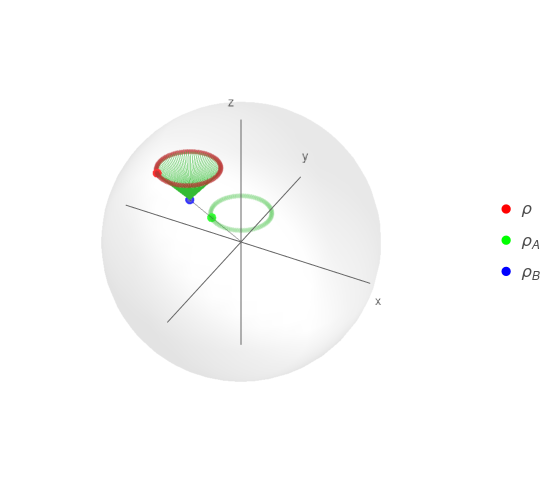
\includegraphics[width=0.6\linewidth]{maxent/figures/U1xU2_H1=sz_H2=Id_z=0.9_p=0.4_sequence.png}
    \caption{En rojo, la evolución temporal del estado efectivo. En verde y azul, $(r_{A}\hat{r}_{\rho})$ y $(r_{B}\hat{r}_{\rho})$ respectivamente.}
    \label{fig:ZRot}
\end{figure}

\subsubsection{Cambio de fase $H=\sigma_{z}$}
Considérese el hamiltoniano $H=\sigma_{z}$. La rotación en la esfera debida a la unitaria generada por el hamiltoniano es una alrededor del eje $z$. La representación de esto, y de el resultado general (\ref{eq:SeparableDynamicsUxIBloch}) puede verse en la figura \ref{fig:ZRot}.


En el espacio de operadores de densidad, esto equivale a insertar una fase relativa en el primer subsistema fino. En efecto, ignorando fases globales,
\begin{equation}
    e^{it\sigma_{z}}=\begin{pmatrix}
        1&0\\0&e^{-i2t}
    \end{pmatrix}
\end{equation}
El estado grueso siente el cambio de fase relativa en su primera componente \notaAd{¿Qué son las trazas del MaxEnt?}.
\begin{equation}
    \rho\xrightarrow{\mcU=e^{it\sigma_{z}}\otimes \Id} p\frac{1}{Z_{1}}e^{it\sigma_{z}}e^{\lambda_{3}p\hat{r}_{\rho}\cdot\vec{\sigma}}e^{-it\sigma_{z}}+(1-p)\frac{1}{Z_{2}}e^{\lambda_{3}(1-p)\hat{r}_{\rho}\cdot\vec{\sigma}}
\end{equation}

\begin{figure}[h!]
    \centering
    \begin{subfigure}{0.32\textwidth}
      \centering
      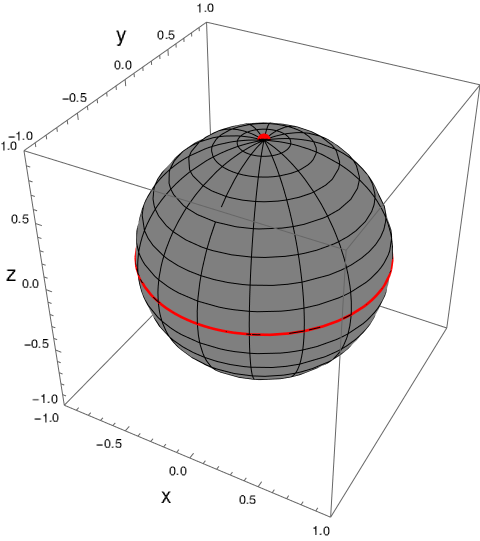
\includegraphics[width=0.9\linewidth]{maxent/figures/U1xU2_H1=Pi(sz)_H2=Id_z=0.9_p=0.6t=0.png}
      \caption{$t=0.0$}
    \end{subfigure}%
    \begin{subfigure}{0.32\textwidth}
      \centering
      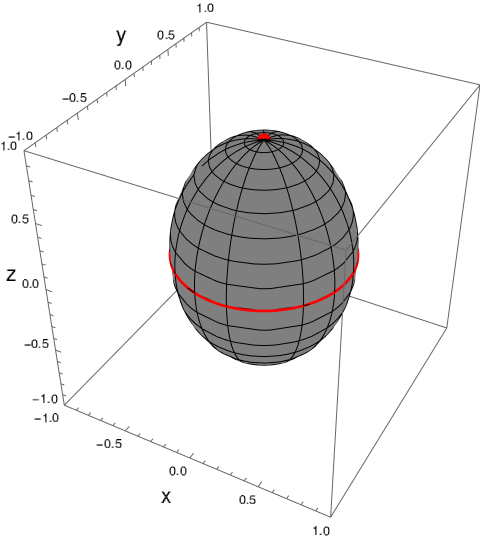
\includegraphics[width=0.9\linewidth]{maxent/figures/U1xU2_H1=Pi(sz)_H2=Id_z=0.9_p=0.6t=0.25.png}
      \caption{$t=0.25$}
    \end{subfigure}
    \begin{subfigure}{0.32\textwidth}
      \centering
      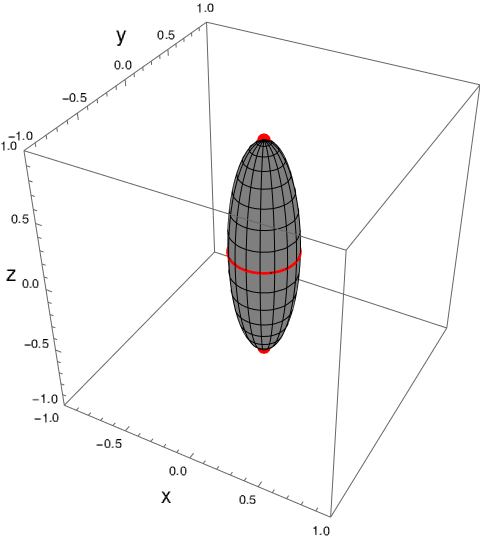
\includegraphics[width=0.9\linewidth]{maxent/figures/U1xU2_H1=Pi(sz)_H2=Id_z=0.9_p=0.6t=0.5.png}
      \caption{$t=0.5$}
    \end{subfigure}
    \caption{Efecto de la evolución subyacente sobre la esfera de Bloch si $r_{z}=0.9$, $p=0.6$ y $U_{1}=e^{it\pi \pauli{3}}$.}
    \label{fig:FaseChangeSequence}
\end{figure}

\subsubsection{Tengo que ver cómo interpreto esta $H=a\sigma_{x}+b\sigma_{y}$}
La transformación es una rotación respecto al eje $(a,b,0)$. Al aplicarse sobre el primer subsistema, el resultado es una rotación de la primera componente del estado grueso. De nuevo, la condición de normalización entre dichas componentes asegura que el estado grueso se mantenga dentro de la esfera de Bloch. 
\begin{figure}[h!]
    \centering
    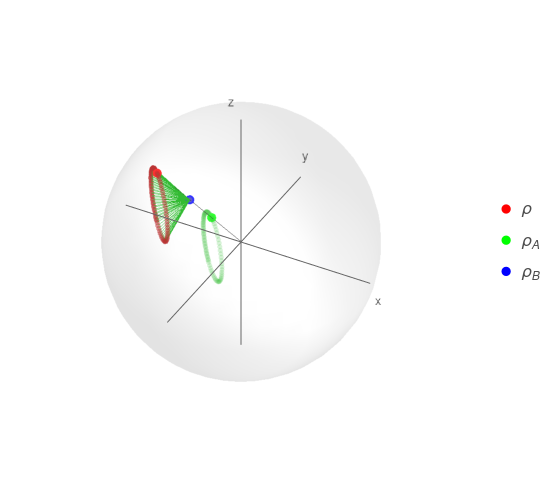
\includegraphics[width=0.6\linewidth]{maxent/figures/U1xU2_H1=sx+sy_H2=Id_z=0.9_p=0.4_sequence.png}
    \caption{En rojo, la evolución temporal del estado efectivo. En verde y azul, $(r_{A}\hat{r}_{\rho})$ y $(r_{B}\hat{r}_{\rho})$ respectivamente. En este ejemplo, $H=\sigma_{x}+2\sigma_{y}$, mientras que $\hat{r}=\frac{0.9}{\sqrt{33}}(-2,-5,2)$}
    \label{fig:XYRot}
\end{figure}

\begin{figure}[h!]
    \centering
    \begin{subfigure}{0.32\textwidth}
      \centering
      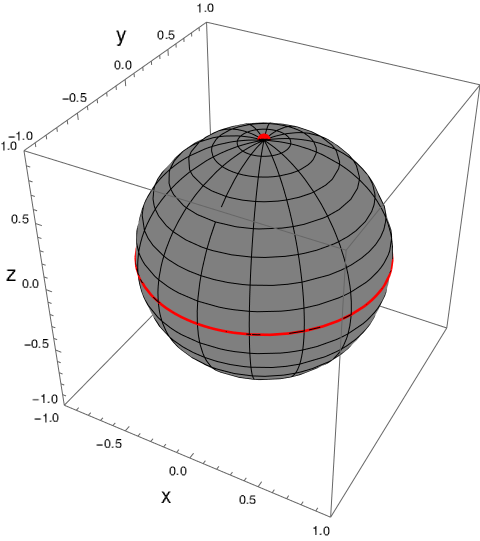
\includegraphics[width=0.9\linewidth]{maxent/figures/U1xU2_H1=Pi(sx+sy)_H2=Id_z=0.9_p=0.6t=0.png}
      \caption{$t=0.0$}
    \end{subfigure}%
    \begin{subfigure}{0.32\textwidth}
      \centering
      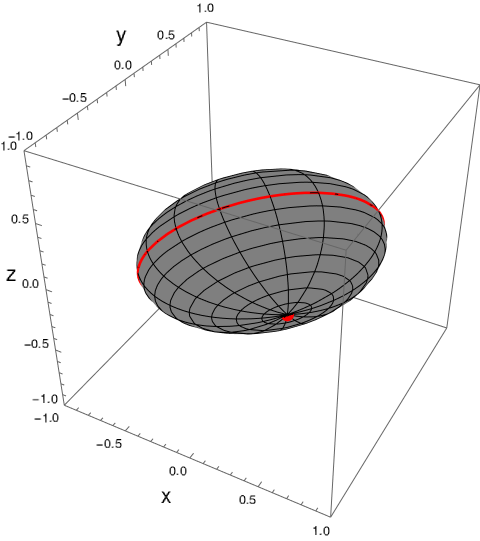
\includegraphics[width=0.9\linewidth]{maxent/figures/U1xU2_H1=Pi(sx+sy)_H2=Id_z=0.9_p=0.6t=0.3.png}
      \caption{$t=0.3$}
    \end{subfigure}
    \begin{subfigure}{0.32\textwidth}
      \centering
      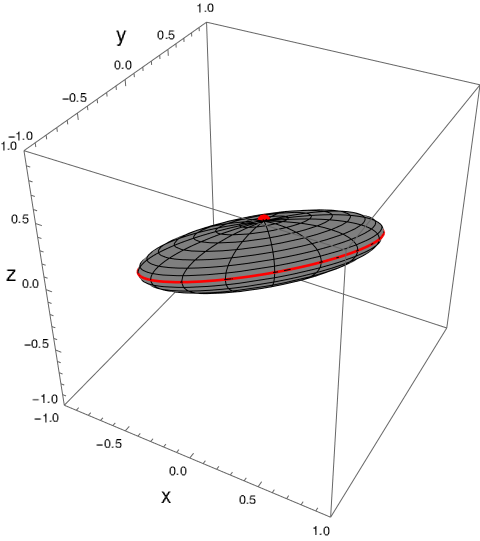
\includegraphics[width=0.9\linewidth]{maxent/figures/U1xU2_H1=Pi(sx+sy)_H2=Id_z=0.9_p=0.6t=0.5.png}
      \caption{$t=0.5$}
    \end{subfigure}
    \caption{Efecto de la evolución subyacente sobre la esfera de Bloch si $r_{z}=0.9$, $p=0.6$ y $U_{1}=e^{it\pi \frac{\pauli{1}+\pauli{2}}{\sqrt{2}}}$.}
    \label{fig:SxSySequence}
\end{figure}

\subsection{El caso $U_{1}=U_{2}=U$}

Quizá el caso más sencillo. La simetría de la unitaria permite factorizarla:
\begin{align*}
\CG{(U^{t}\otimes U^{t})\varrho_{max}(U^{t}\otimes U^{t})^{\dag}}&=p\frac{1}{Z_{1}}e^{\lambda p U^{t}\sigma_{z}(U^t)^{\dag}}+(1-p)\frac{1}{Z_{2}}e^{\lambda (1-p)U^{t}\sigma_{z}(U^t)^{\dag}}\\
&=p\frac{1}{Z_{1}}U^{t}e^{\lambda p \sigma_{z}}(U^t)^{\dag}+(1-p)\frac{1}{Z_{2}}U^{t}e^{\lambda (1-p)\sigma_{z}}(U^t)^{\dag}\\
&=U^{t}\qty(p\frac{1}{Z_{1}}e^{\lambda p \sigma_{z}}+(1-p)\frac{1}{Z_{2}}e^{\lambda (1-p)\sigma_{z}})(U^t)^{\dag}\\
\end{align*}
La dinámica efectiva tiene la forma:
\begin{equation}
    \rho\xrightarrow{U\otimes U}U\rho U^{\dagger}
\end{equation}


\subsection{Límite $(1-p)$ pequeña}
El caso $p\rightarrow 1$ puede interpretarse como aquel en el que el aparato de medición tiene una baja probabilidad de fallar (poco ruido). Las evoluciones separables $U=U_{1}\otimes U_{2}$ pueden verse como una evolución gruesa $U_{1}$ más una perturbación. La perturbación, al ser unitaria, es también una rotación, así que lo que se observa es una especie de hélice. El estado precesa alrededor de una traslación de la que sería su trayectoria no perturbada. Siempre que $U_{2}=\Id$ lo que se observa es una traslación en dirección del estado con magnitud $r_{B}$. Si, por el contrario, $U_{1}=\Id$, una vez más el estado grueso se ve desplazado, para luego comenzar a girar según la rotación inducida por la unitaria $U_{2}$. 

Algunos ejemplos pueden verse en las figuras siguientes.

\begin{figure}[h!]
    \centering
    \begin{subfigure}{0.32\textwidth}
      \centering
      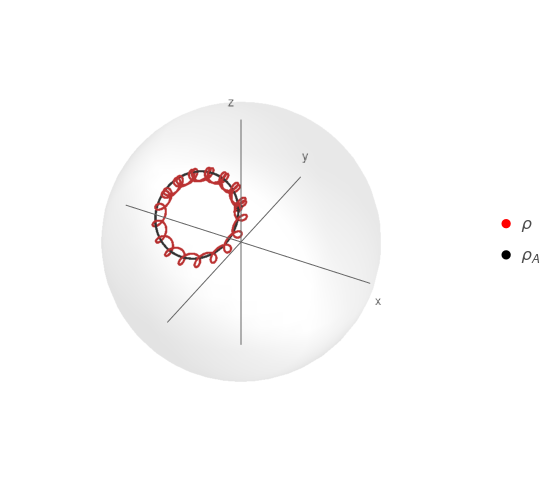
\includegraphics[width=0.9\linewidth]{maxent/figures/U1xU2_H1=(sy-sz)_H2=10(2sx-sy)_z=0.9_p=0.9.png}
      \caption{$t=0.0$}
    \end{subfigure}%
    \begin{subfigure}{0.32\textwidth}
      \centering
      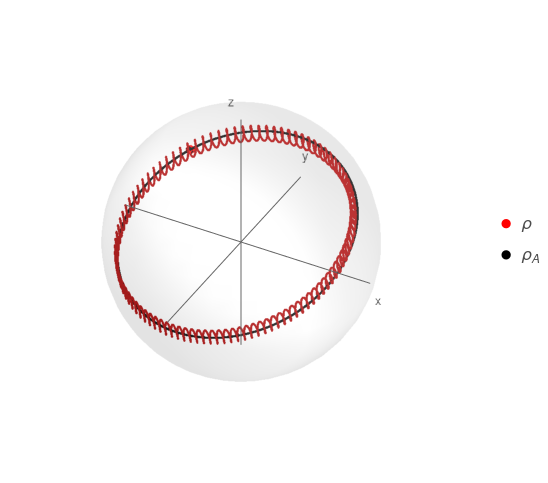
\includegraphics[width=0.9\linewidth]{maxent/figures/U1xU2_H1=(sx-sy)_H2=100(sx+sy)_z=0.9_p=0.9.png}
      \caption{$t=0.3$}
    \end{subfigure}
    \begin{subfigure}{0.32\textwidth}
      \centering
      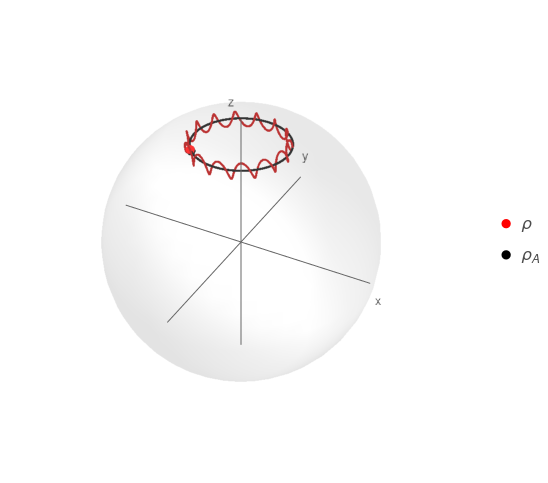
\includegraphics[width=0.9\linewidth]{maxent/figures/U1xU2_H1=sz_H2=10(sx+sy)_z=0.9_p=0.9.png}
      \caption{$t=0.5$}
    \end{subfigure}
    \caption{Efecto de la evolución subyacente sobre la esfera de Bloch si $r_{z}=0.9$, $p=0.6$ y $U_{1}=e^{it\pi \frac{\pauli{1}+\pauli{2}}{\sqrt{2}}}$.}
    \label{fig:NoErrorEvolution}
\end{figure}

\begin{figure}[h!]
    \centering
    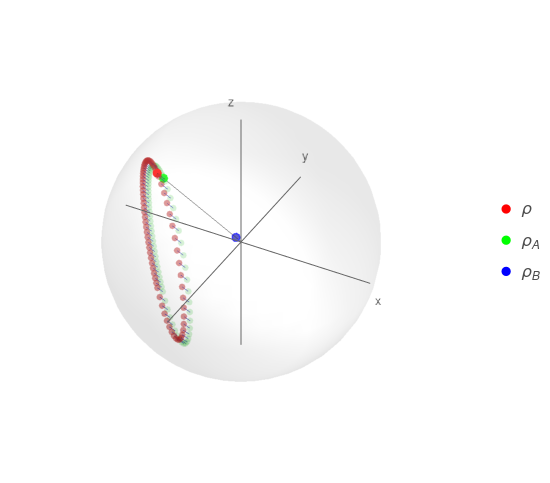
\includegraphics[width=0.6\linewidth]{maxent/figures/U1xU2_H1=(sx+sy)_H2=Id_z=0.9_p=0.85_sequence.png}
    \caption{Este es el caso $H_{1}=(\sigma_{x}+\sigma_{y})$ y $H_{2}=\Id$. El resultado de la perturbación es una traslación en la evolución del estado.}
    \label{fig:SmallP1}
\end{figure}


\begin{figure}[h!]
    \centering
    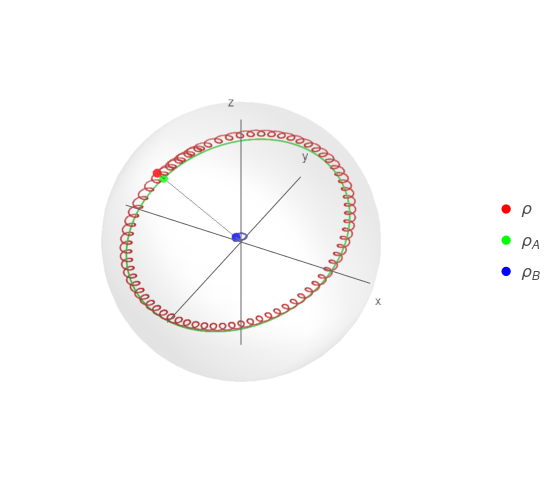
\includegraphics[width=0.6\linewidth]{maxent/figures/U1xU2_H1=100(sx-sy)_H2=sz_z=0.9_p=0.85_sequence.png}
    \caption{Este es el caso $H_{1}=100(\sigma_{x}-\sigma_{y})$ y $H_{2}=\sigma_{z}$. Las oscilaciones alrededor de la óribita desplazada son visibles.}
    \label{fig:SmallP2}
\end{figure}

\begin{figure}[h!]
    \centering
    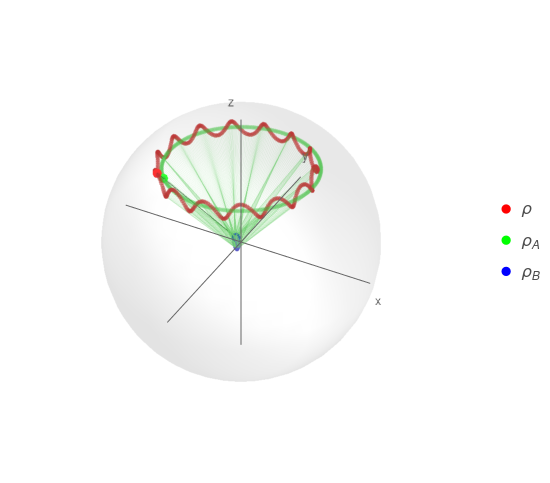
\includegraphics[width=0.6\linewidth]{maxent/figures/U1xU2_H1=sz_H2=10*(sx+sy)_z=0.9_p=0.85_sequence.png}
    \caption{Este es el caso $H_{1}=\sigma_{z}$ y $H_{2}=10(\sigma_{x}+\sigma_{y})$. Las oscilaciones alrededor de la óribita desplazada son visibles.}
    \label{fig:SmallP3}
\end{figure}


\newpage
\section{Modelo de Ising}


El Hamiltoniano del modelo de Ising transversal es
\begin{equation*}
    H=-\omega\qty(\sum_{\langle j,k \rangle}\pauli{3,j}\otimes\pauli{3,k}+g\sum_{k}\Id\otimes\pauli{1,k}),
\end{equation*}

que, si $g=0$ (fase ordenada) y tomando en cuenta únicamente un par de partículas se convierte en el Hamiltoniano de interacción
\begin{equation*}
    H=-\omega \pauli{3}\otimes\pauli{3}.
\end{equation*}

Dado un estado efectivo $\rho\in\densityspace{2}$, propagar al estado asignando a través del Principio de Máxima Entropía con dicha evolución y luego tomar la descripción dada por la aplicación de grano grueso resulta en la dinámica efectiva
\begin{align*}
    \Gamma_{t}^{p}(\rho)=&\rho \cos^{2}(\omega)+\pauli{3} \rho \pauli{3} \sin^{2}(\omega t)\\
    & + i\sin(\omega t)\cos(\omega t)\qty(p\expval{\pauli{3}}_{B}[\pauli{3},\rho_{A}]+(1-p)\expval{\pauli{3}}_{A}[\pauli{3},\rho_{B}]).
\end{align*}
Reconocemos dos términos: uno lineal y uno no lineal. El primero tiene forma de canal de desfasamiento sobre el estado efectivo. El segundo depende de los parámetros de la aplicación de grano grueso y de los valores esperados con respecto a los operadores de densidad reducidos del estado de máxima entropía. En efecto, el caso límite $p=1$ o $p=1$ simplemente reduce la dinámica a un canal de desfasamiento:

\begin{equation*}
    \Gamma_{t}^{p=1}(\rho)=\rho \cos^{2}(\omega)+\pauli{3} \rho \pauli{3} \sin^{2}(\omega t).
\end{equation*}

mientras que el caso $p=\frac{1}{2}$ revela el efecto del término no lineal:

\begin{equation*}
    \Gamma_{t}^{p=\frac{1}{2}}(\rho)=\rho \cos^{2}(\omega)+\pauli{3} \rho \pauli{3} \sin^{2}(\omega t) + i\expval{\pauli{3}} \qty[\pauli{3},\rho] \sin(\omega t)\cos(\omega t).
\end{equation*}

Nótese que, si del factor $\expval{\pauli{3}}=1$, la dinámica sería no solo lineal, sino unitaria, y correspondería a una rotación respecto al eje $z$, de no ser que los únicos estados tales que $\expval{\pauli{3}}=1$ son invariantes bajo dichas rotaciones. En realidad, lo que se observa es que la dinámica efectiva es una rotación respecto a $z$ que depende de la componente en $z$ del estado efectivo inicial. Cuando $\expval{\pauli{3}}=0$, la dinámica es un canal de despolarización que manda a todos los estados al eje $z$ (a un tiempo $\omega t =\frac{\pi}{4}$). 

\begin{figure}[ht!]
    \centering
    \begin{subfigure}{0.32\textwidth}
      \centering
      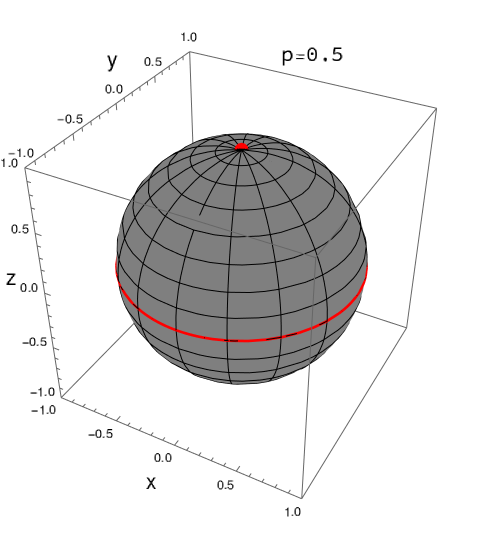
\includegraphics[width=0.9\linewidth]{../thesis/chapter3/figures_special/sphere_Ising_t=0._z=0.9_p=0.5.png}
      \caption{$t=0$}
    \end{subfigure}%
    \begin{subfigure}{0.32\textwidth}
      \centering
      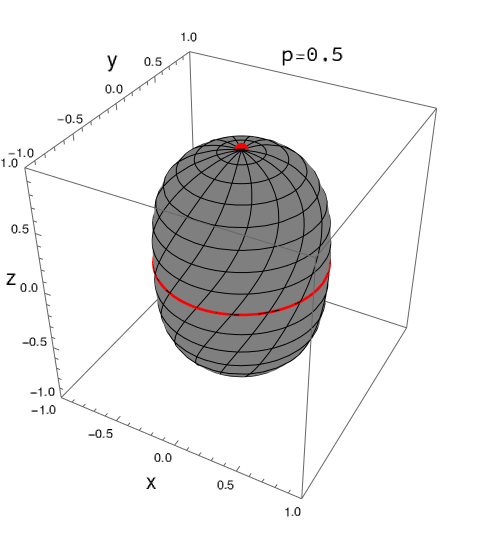
\includegraphics[width=0.9\linewidth]{../thesis/chapter3/figures_special/sphere_Ising_t=0.5_z=0.9_p=0.5.png}
      \caption{$t=0.5$}
    \end{subfigure}
    \begin{subfigure}{0.32\textwidth}
      \centering
      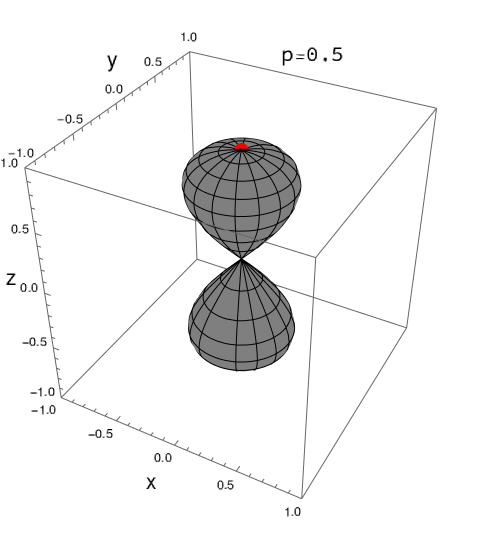
\includegraphics[width=0.9\linewidth]{../thesis/chapter3/figures_special/sphere_Ising_t=1._z=0.9_p=0.5.png}
      \caption{$t=1$}
    \end{subfigure}
    \caption{Efecto del la evolución sobre la esfera de Bloch cuando $p=\frac{1}{2}$. Nótese que el desfasamiento sólo se completa en el eje $xy$.}
    \label{fig:Ising_p0.5_Sequence}
    \end{figure}

La despolarización dependiente de la componente en $z$ inicial es más clara si se observa el efecto de la evolución sobre el vector de Bloch. Abusando un poco de la notación se nota que 

\begin{equation*}
    \Gamma_{t}^{p=\frac{1}{2}}(\vec{r}_{\rho})=\begin{pmatrix}
        x\cos(2\omega t)-yz\sin(2\omega t)\\
        y\cos(2\omega t)+xz(2\omega t)\\
        z\\
    \end{pmatrix}
\end{equation*}
\acnote{Aquí se ve la casi rotación, pero creo que lo tengo que descomponer en diferentes operaciones para notar que el desfasamiento se da de forma más fuerte conforme más pequeño es z}
\section{Canal de despolarización}


Consideremos una evolución subyacente no unitaria: el canal de despolarización. El canal de despolarización para $n$ partículas está definido como
\begin{equation*}
    D_{\mu}(\varrho)=\mu\varrho+(1-\mu)\Id.
\end{equation*}
Dado un estado efectivo inicial $\rho$, su asignación de máxima entropía es $\varrho_{\max}=\rho_{A}\otimes\rho_{B}$. El resultado de pasar al estado de máxima entropía por el canal de despolarización es simplemente
\begin{equation*}
    D_{\mu}(\varrho_{\max})=\mu\varrho_{\max}+(1-\mu)\Id.
\end{equation*}
Esto significa que la dinámica efectiva es
\begin{equation*}
    \Gamma_{t=1}(\rho)=\mu\rho+(1-\mu)\Id,
\end{equation*}
esto es, ¡el mismo canal de despolarización aplicado a un sistema de menos partículas! Nótese que este resultado es muy similar al obtenido para una evolución unitaria subyacente generada por un Hamiltoniano de la forma $\mcH=H\otimes\Id+\Id\otimes H$. En dicho caso, la dinámica efectiva era, justamente, la unitaria generada por el Hamiltoniano $H$, esto como consecuencia de la simetría de la evolución: la misma para cada partícula, sin interacción. Este caso es el mismo, el canal de despolarización actúa de la misma forma sobre cada partícula, y es completamente isotrópico dentro del subespacio de cada partícula.
\section{Decaimientos}

\subsection{Estabilización espontánea ?}
Considérese que un sistema de $n$ partículas evoluciona siguiendo el canal
\begin{equation*}
    \mcE_{\psi,t}[\varrho]=e^{-t\mu}\varrho+(1-e^{-t \mu})\dyad{\psi}
\end{equation*}
donde $\dyad{\psi}\in \densityspace{n}$. Aplicando el modelo de grano grueso se obtiene que:
\begin{equation*}
    \rho(t)=e^{-t\mu}\rho(0)+(1-e^{-t \mu})\dyad{\psi}_{eff}
\end{equation*}
donde $\dyad{\psi}_{eff}=\mcC(\dyad{\psi})$. Obsérvese que el resultado es un canal del mismo tipo. La única diferencia siendo que el estado al que el sistema \textit{decae} (abusando del lenguaje) es la descripción efectiva de $\dyad{\psi}$. Como es natural, el comportamiento de la evolución es completamente dependiente de $\psi$, pero, al fin y al cabo, ¡se obtiene un canal cuántico!

\subsection{Amortiguamiento de amplitud}


\newpage


\bibliographystyle{ieeetr}
\bibliography{bibliography}


\end{document}
